\section*{Figure Legends}
\label{figures}

\subsubsection*{Figure~\ref{fig:chondrocyte-model}.}
An illustration of the model.

\subsubsection*{Figure~\ref{fig:background-currents-vi}.}
The background currents (ramped voltage (over 1~s) vs. current).

\subsubsection*{Figure~\ref{fig:pumps-and-exchangers-vi}.}
The different pumps and exchanger currents (ramped voltage (over 1~s) vs. current).

\subsubsection*{Figure~\ref{fig:potassium-currents-vi}.}
The other potassium currents (ramped voltage (over 1~s)
vs. current). Experimental values (in red) from \cite{Clarketal2011}.

\subsubsection*{Figure~\ref{fig:other-currents-vi}.}
All other currents (V-I). Disabled until we determine exact
channels/functional forms.

\subsubsection*{Figure~\ref{fig:concentrations}.}
Evolution of the concentrations over 2000~s.

\subsubsection*{Figure~\ref{fig:background-currents-ti}.}
Evolution of the background currents over 2000~s.

\subsubsection*{Figure~\ref{fig:pumps-and-exchangers-ti}.}
Evolution of the different pump and exchanger currents over 2000~s.

\subsubsection*{Figure~\ref{fig:potassium-currents-ti}.}
Evolution of the other potassium currents over 2000~s.

\subsubsection*{Figure~\ref{fig:other-currents-ti}.}
Evolution of all the other currents over 2000~s. (Currently disabled.)

\subsubsection*{Figure~\ref{fig:overall-behaviour}.}
Overall behaviour of the model.

\subsubsection*{Figure~\ref{fig:varying-Ko}.}
Evolution of membrane potential with varying external potassium concentration.

\clearpage
\begin{figure}
  \centering
  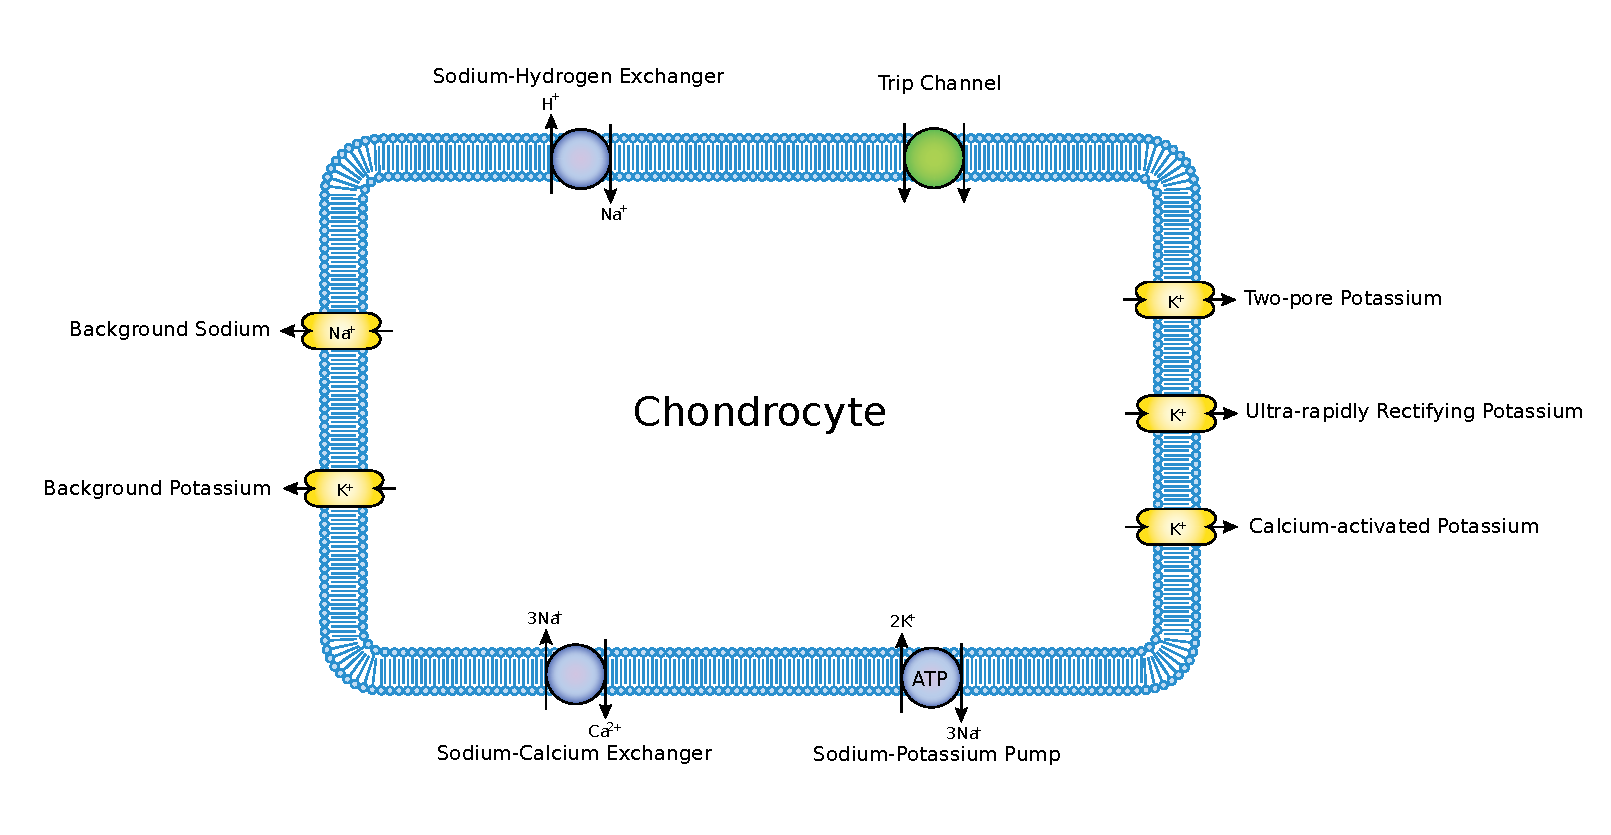
\includegraphics[width=\textwidth]
  {../images/pdf/chondrocyte-model-cellml}
  \caption{}
  \label{fig:chondrocyte-model}
\end{figure}

\clearpage
\begin{figure}
  \centering
  \subfloat{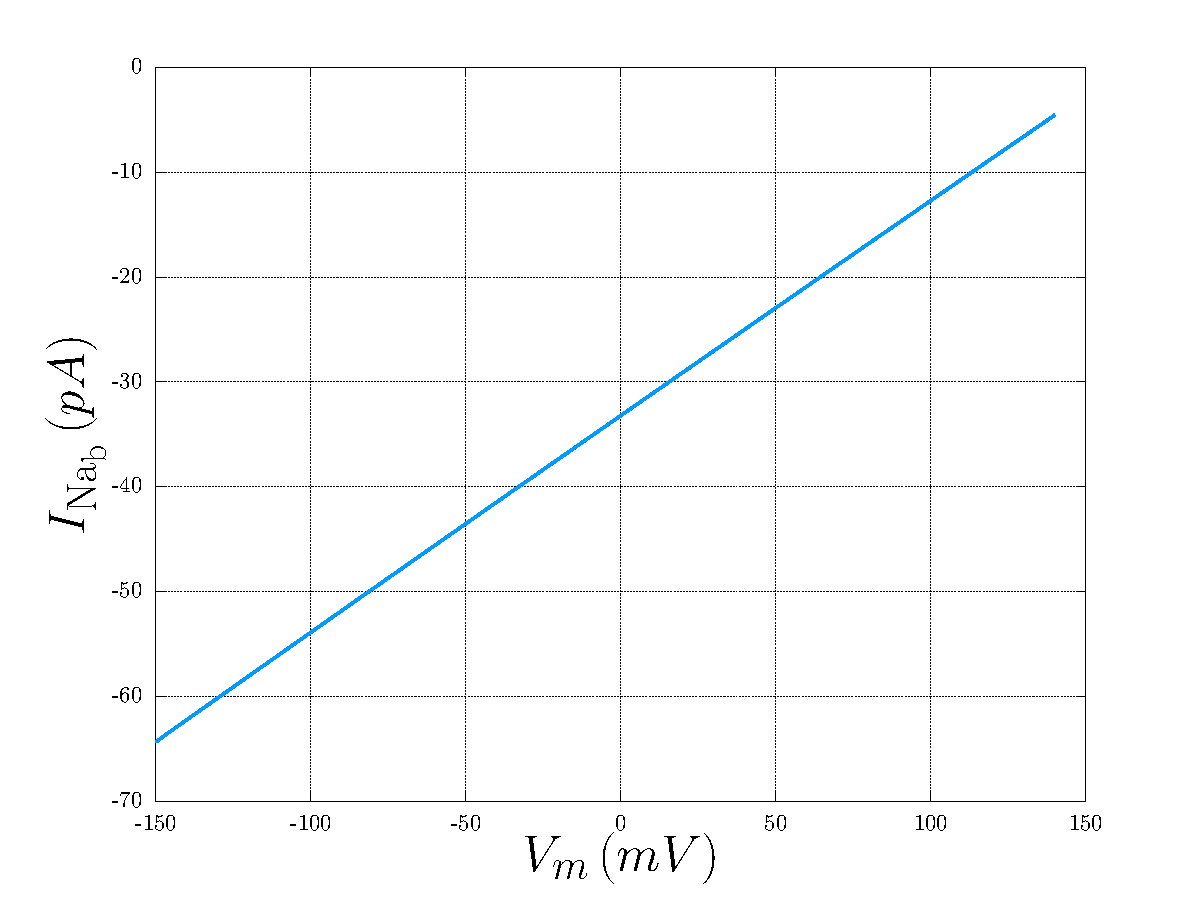
\includegraphics[width=0.36\textwidth]
    {../results/pdf/20110902/V-I_Na_b}}
  \subfloat{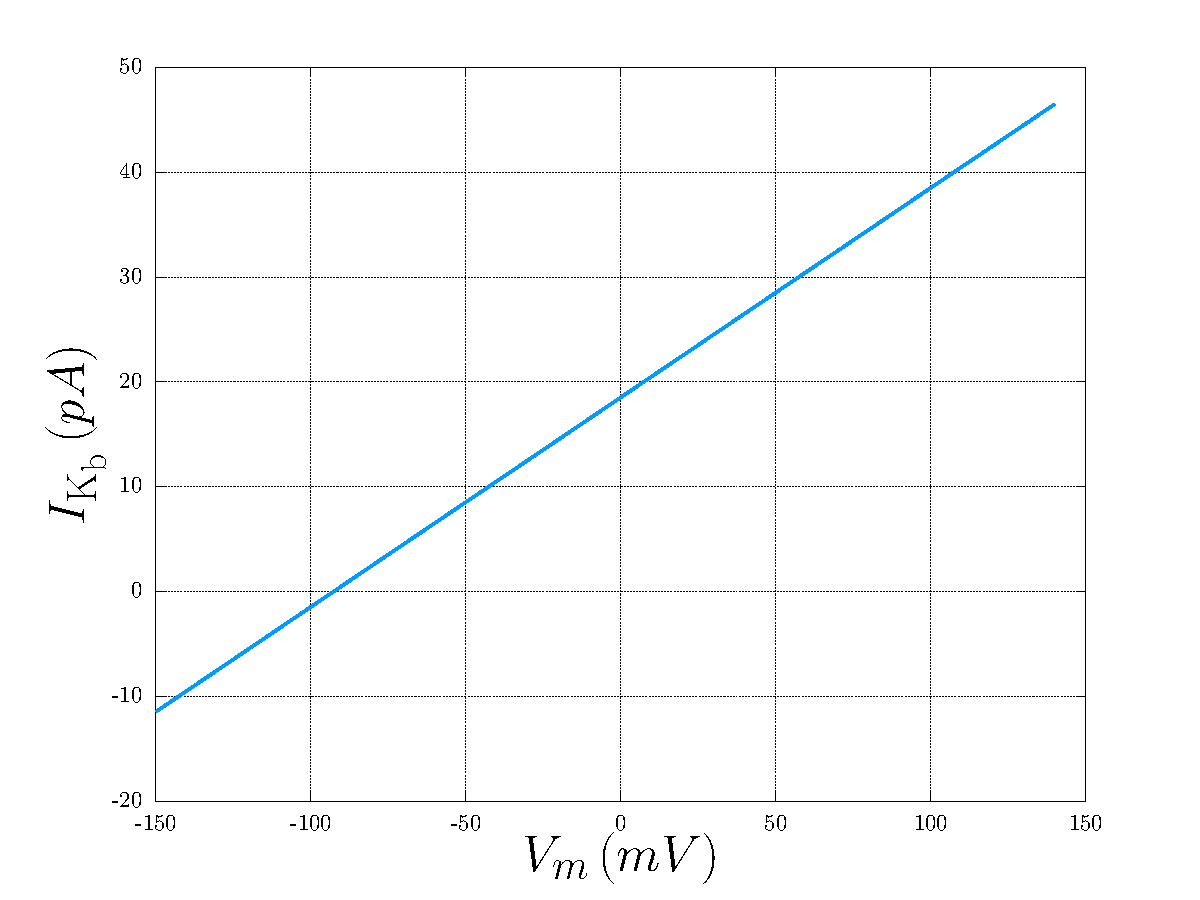
\includegraphics[width=0.36\textwidth]
    {../results/pdf/20110902/V-I_K_b}}\\
  \subfloat{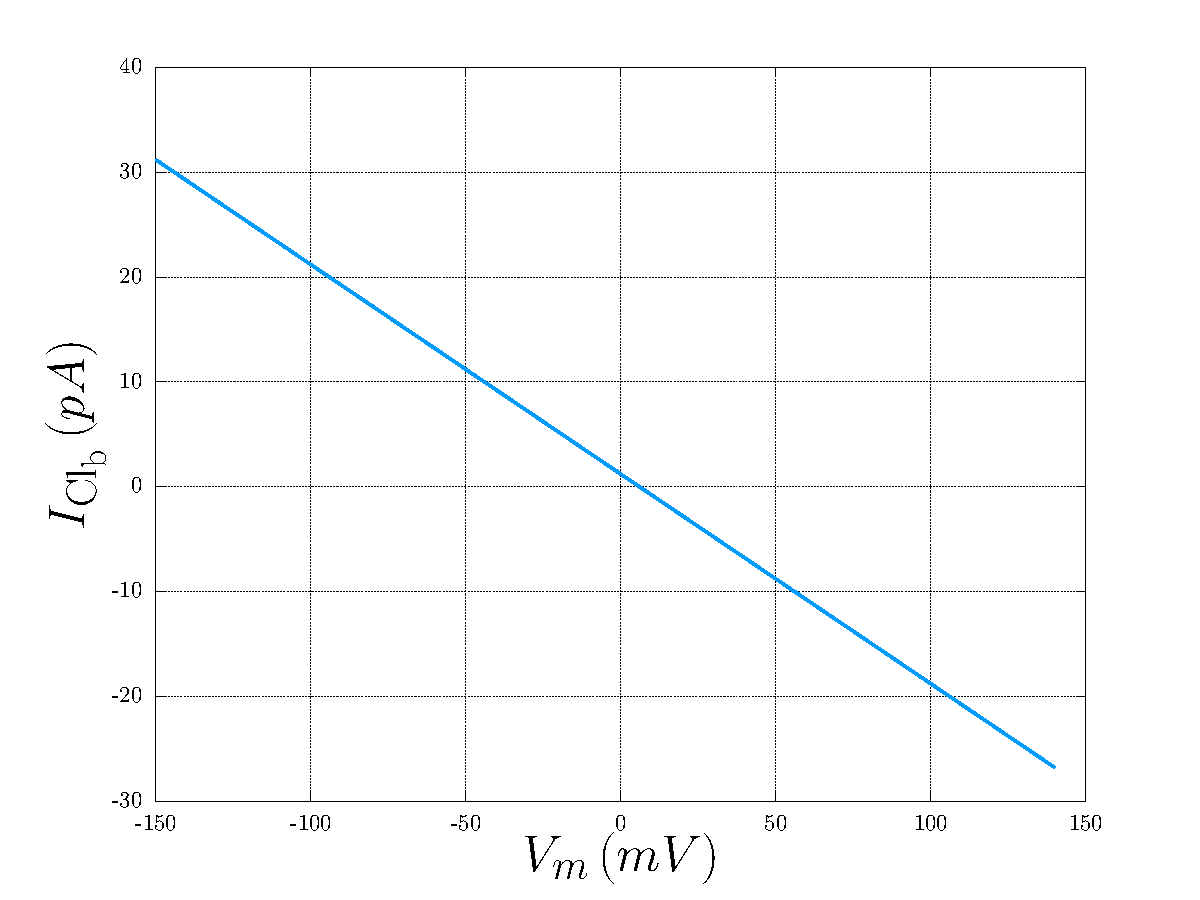
\includegraphics[width=0.36\textwidth]
    {../results/pdf/20110902/V-I_Cl_b}}
  \subfloat{\hspace{0.36\textwidth}}
  \caption{}
  \label{fig:background-currents-vi}
\end{figure}

\clearpage
\begin{figure}
  \centering
  \subfloat{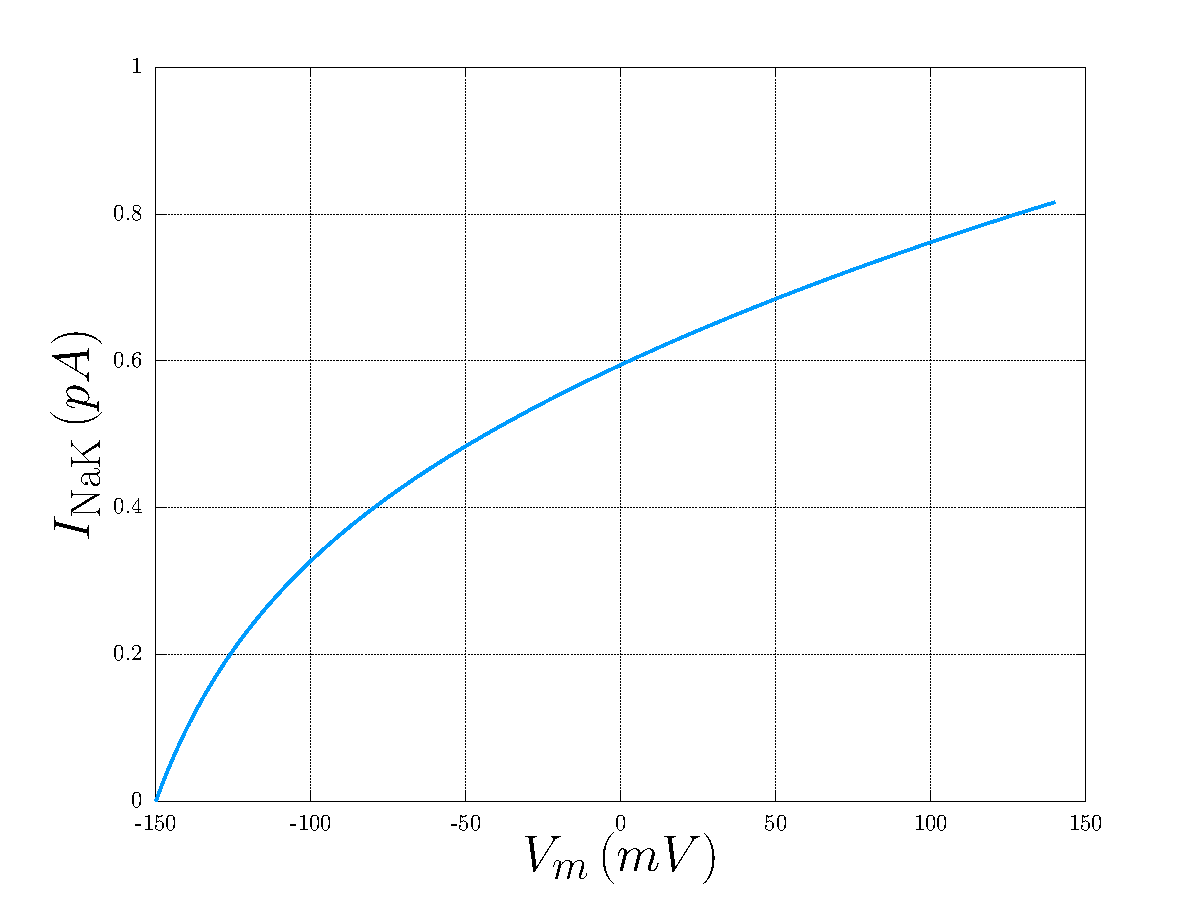
\includegraphics[width=0.36\textwidth]
    {../results/pdf/20110902/V-I_NaK}}
  \subfloat{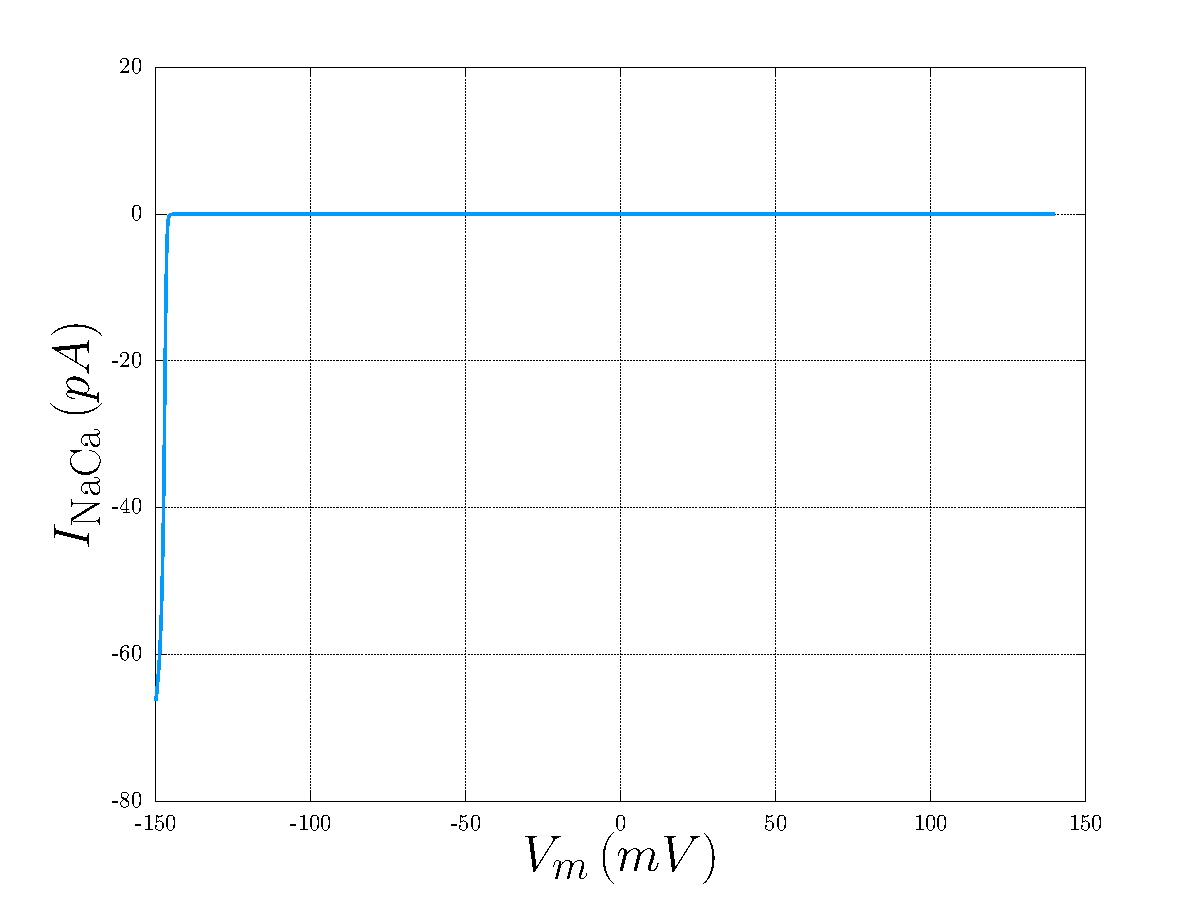
\includegraphics[width=0.36\textwidth]
    {../results/pdf/20110902/V-I_NaCa}}\\
  \subfloat{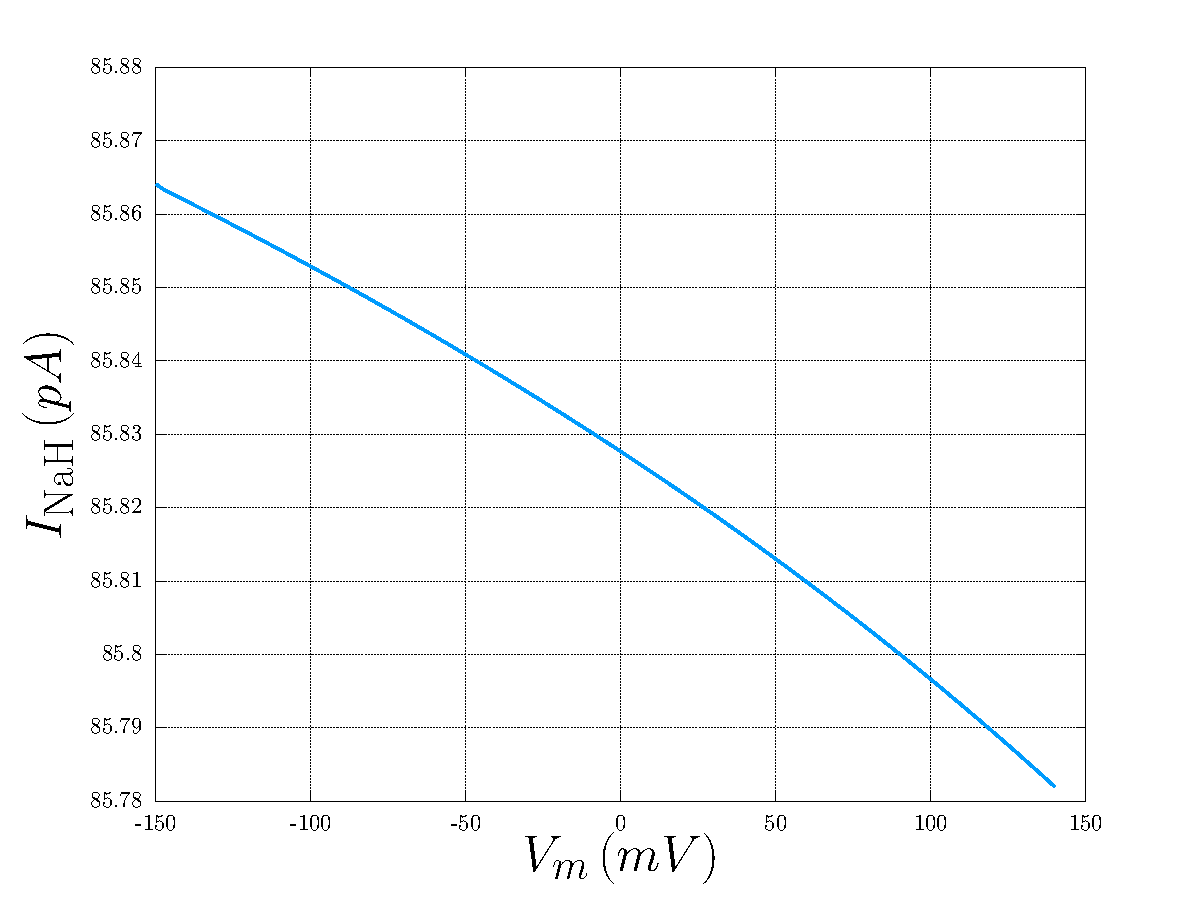
\includegraphics[width=0.36\textwidth]
    {../results/pdf/20110902/V-I_NaH}}
  \subfloat{\hspace{0.36\textwidth}}
  \caption{}
  \label{fig:pumps-and-exchangers-vi}
\end{figure}

\clearpage
\begin{figure}
  \centering
  \subfloat{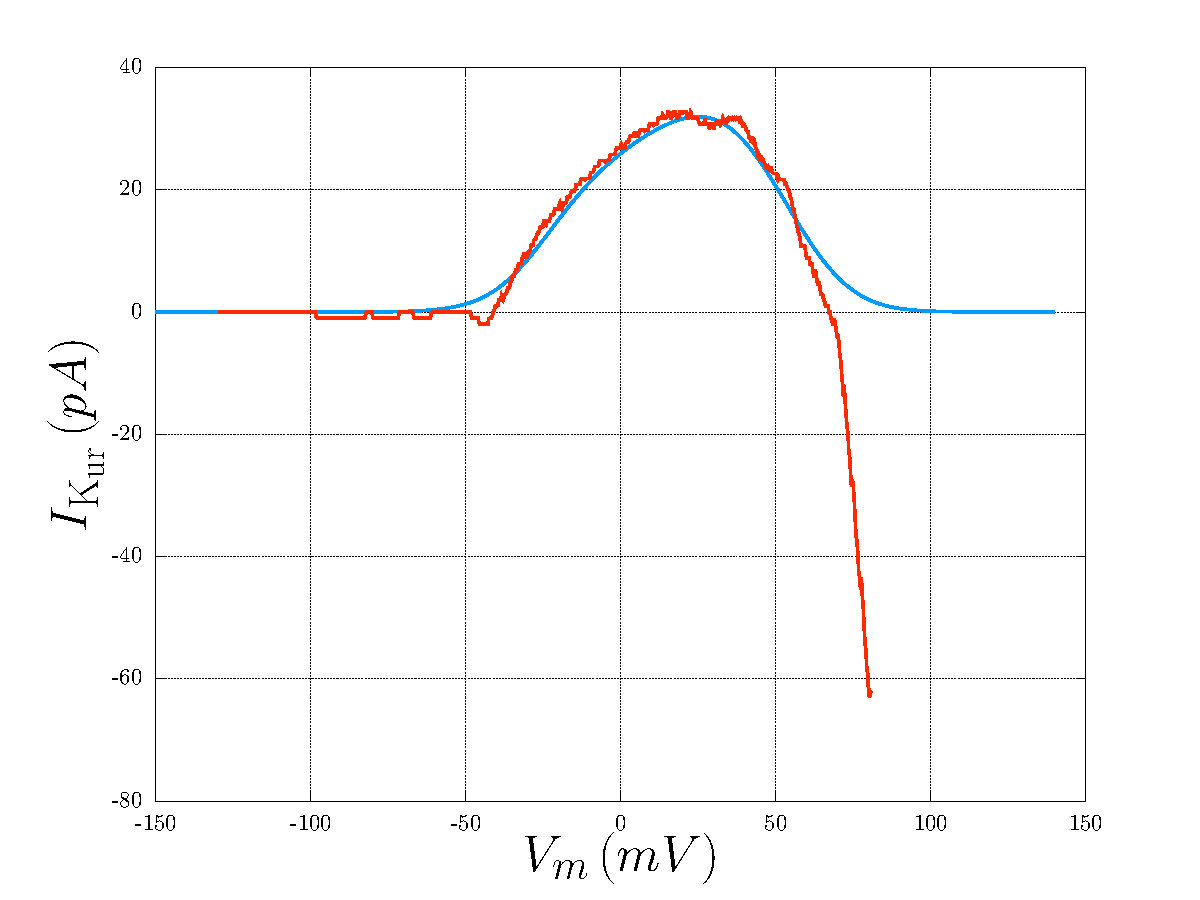
\includegraphics[width=0.36\textwidth]
    {../results/pdf/20110902/V-I_K_ur}}
  \subfloat{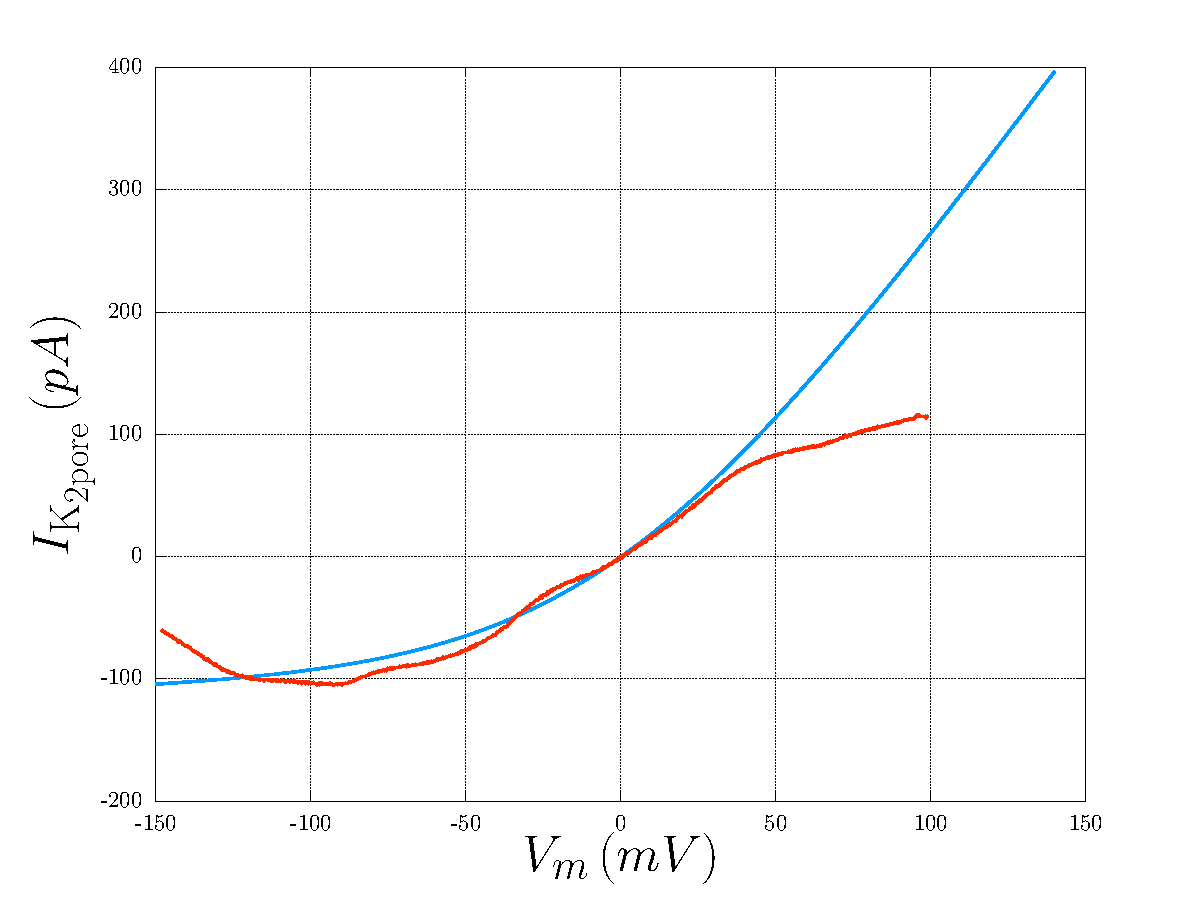
\includegraphics[width=0.36\textwidth]
    {../results/pdf/20110902/V-I_K_2pore}}\\
  \subfloat{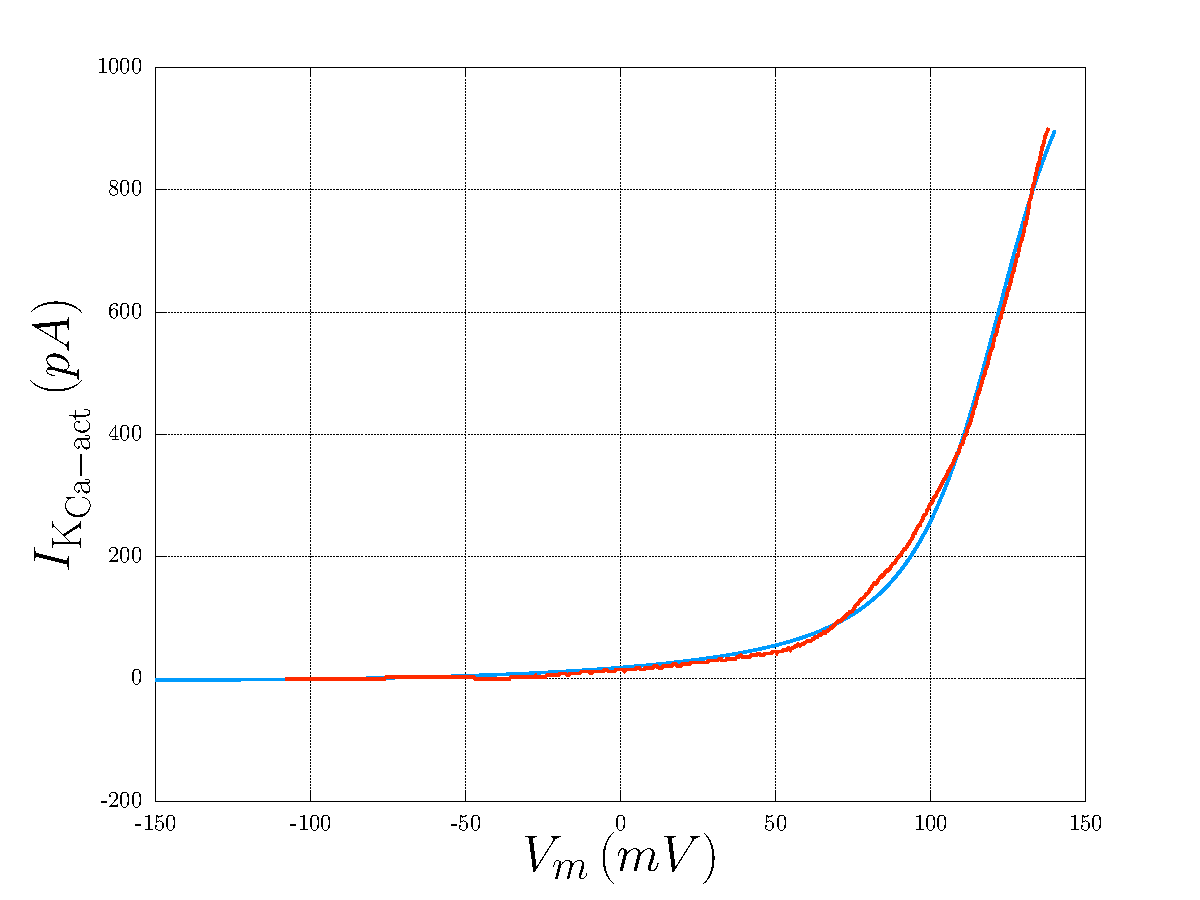
\includegraphics[width=0.36\textwidth]
    {../results/pdf/20110902/V-I_K_Ca_act}}
  \subfloat{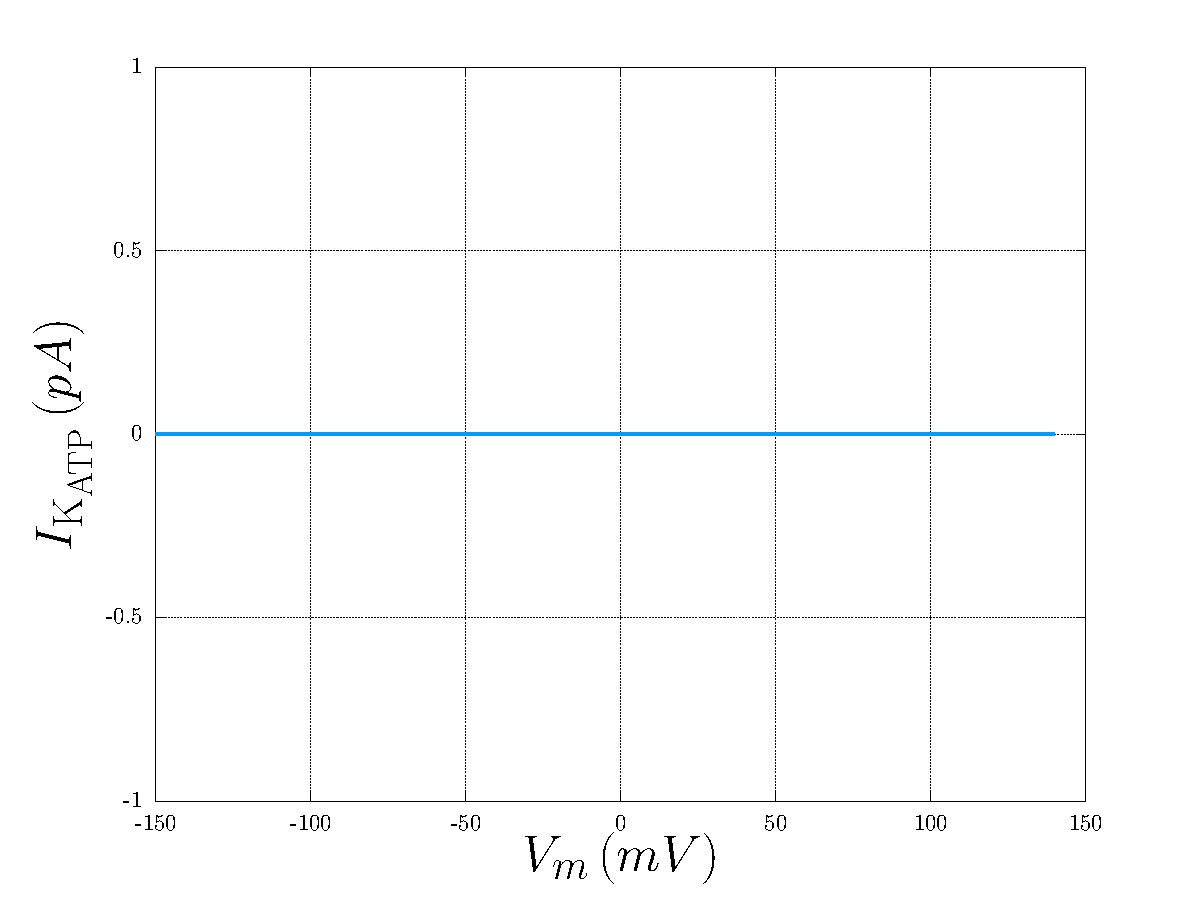
\includegraphics[width=0.36\textwidth]
    {../results/pdf/20110902/V-I_K_ATP}}
  \caption{}
  \label{fig:potassium-currents-vi}
\end{figure}

\clearpage
\begin{figure}
  \centering
  \subfloat{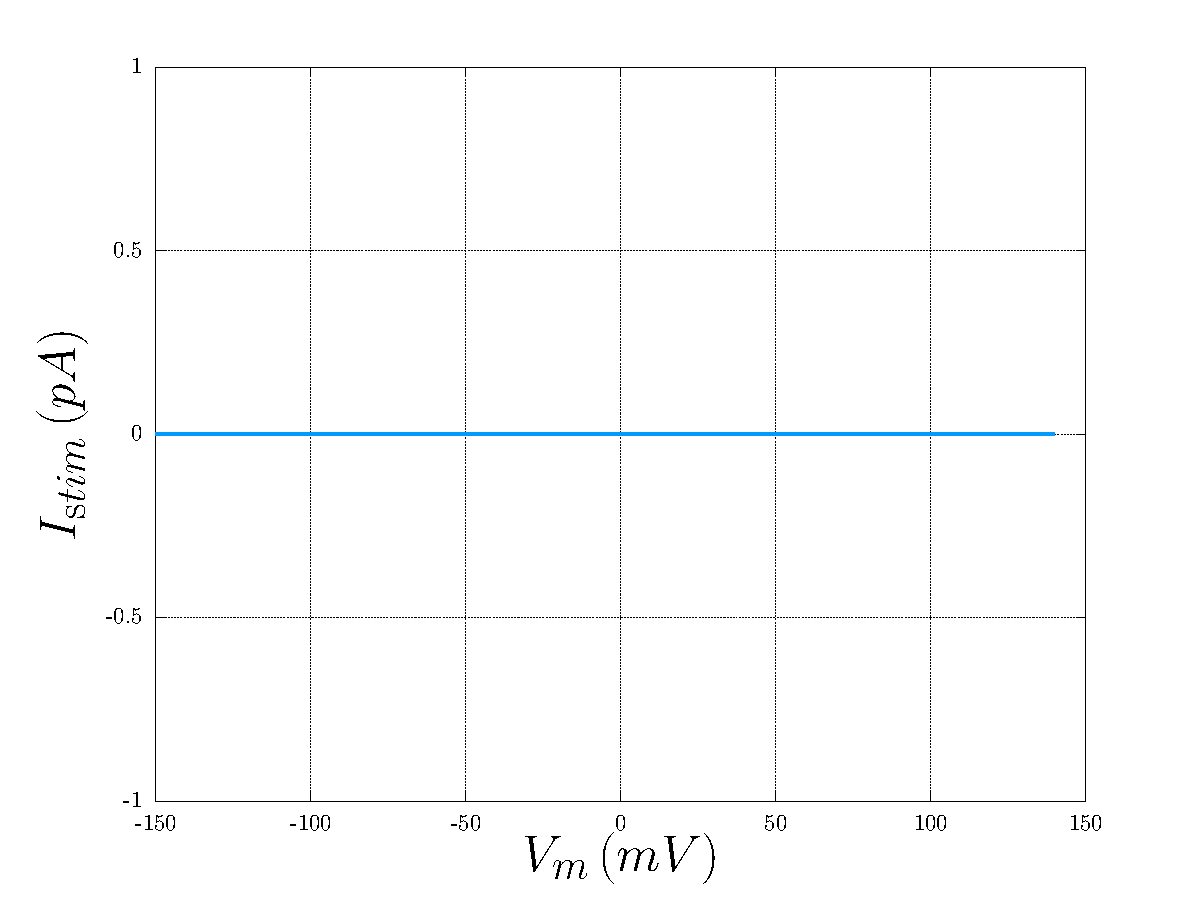
\includegraphics[width=0.36\textwidth]
    {../results/pdf/20110902/V-I_stim}}
  \subfloat{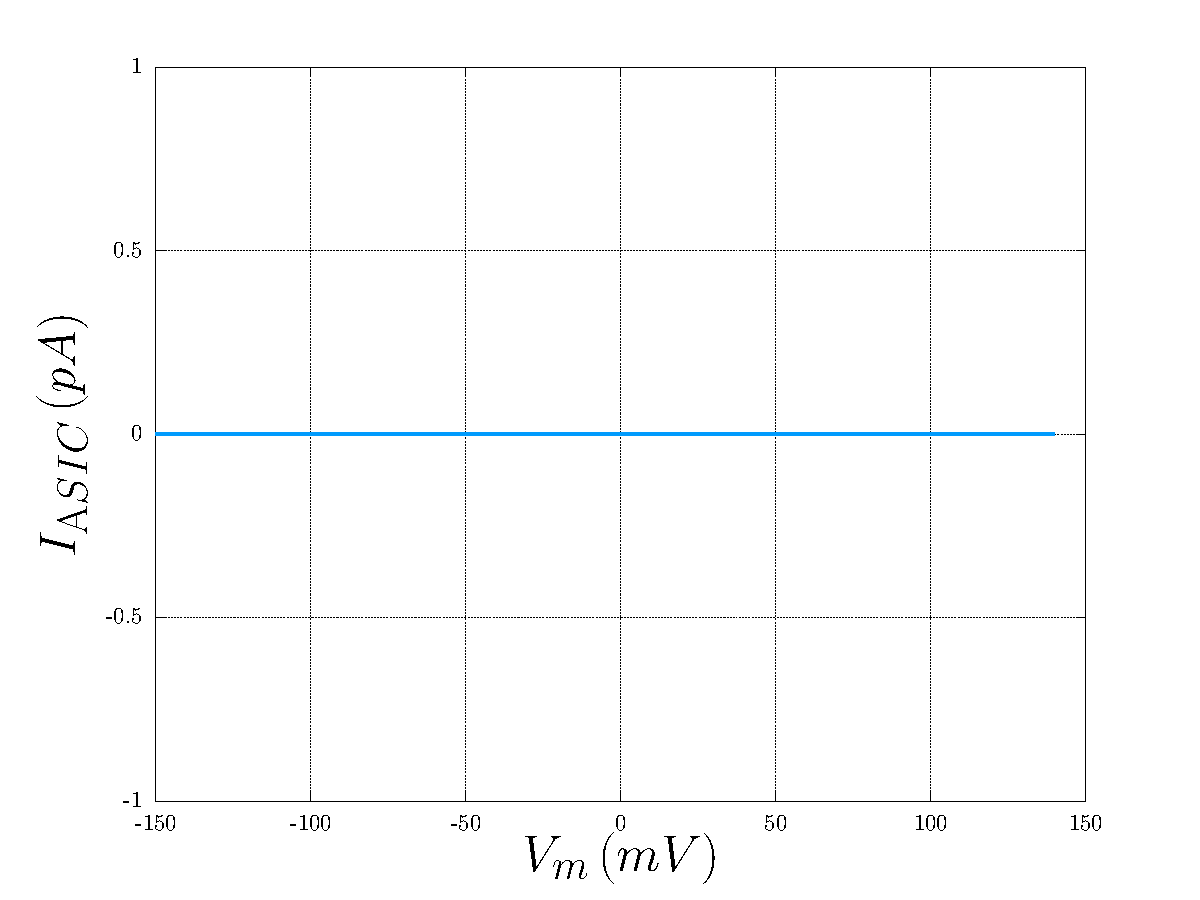
\includegraphics[width=0.36\textwidth]
    {../results/pdf/20110902/V-I_ASIC}}\\
  \subfloat{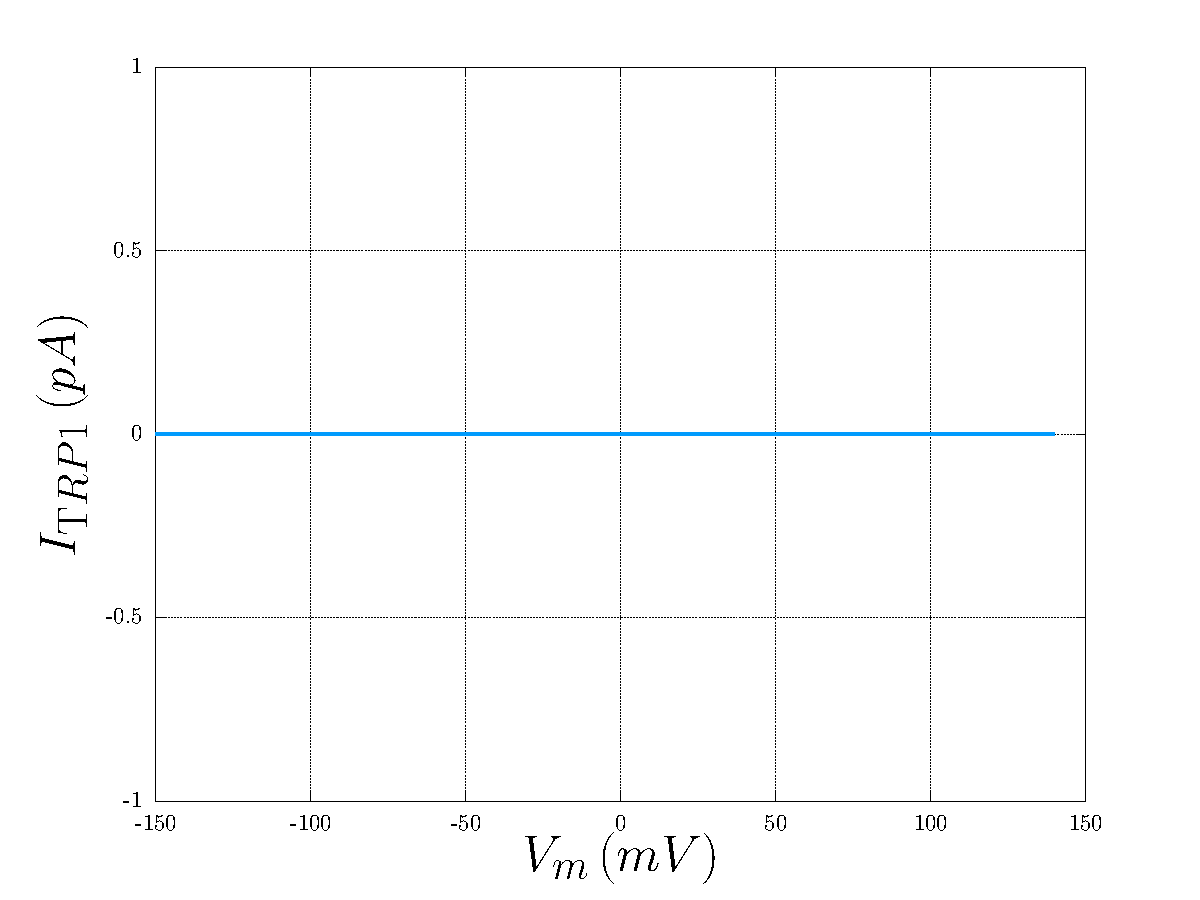
\includegraphics[width=0.36\textwidth]
    {../results/pdf/20110902/V-I_TRP1}}
  \subfloat{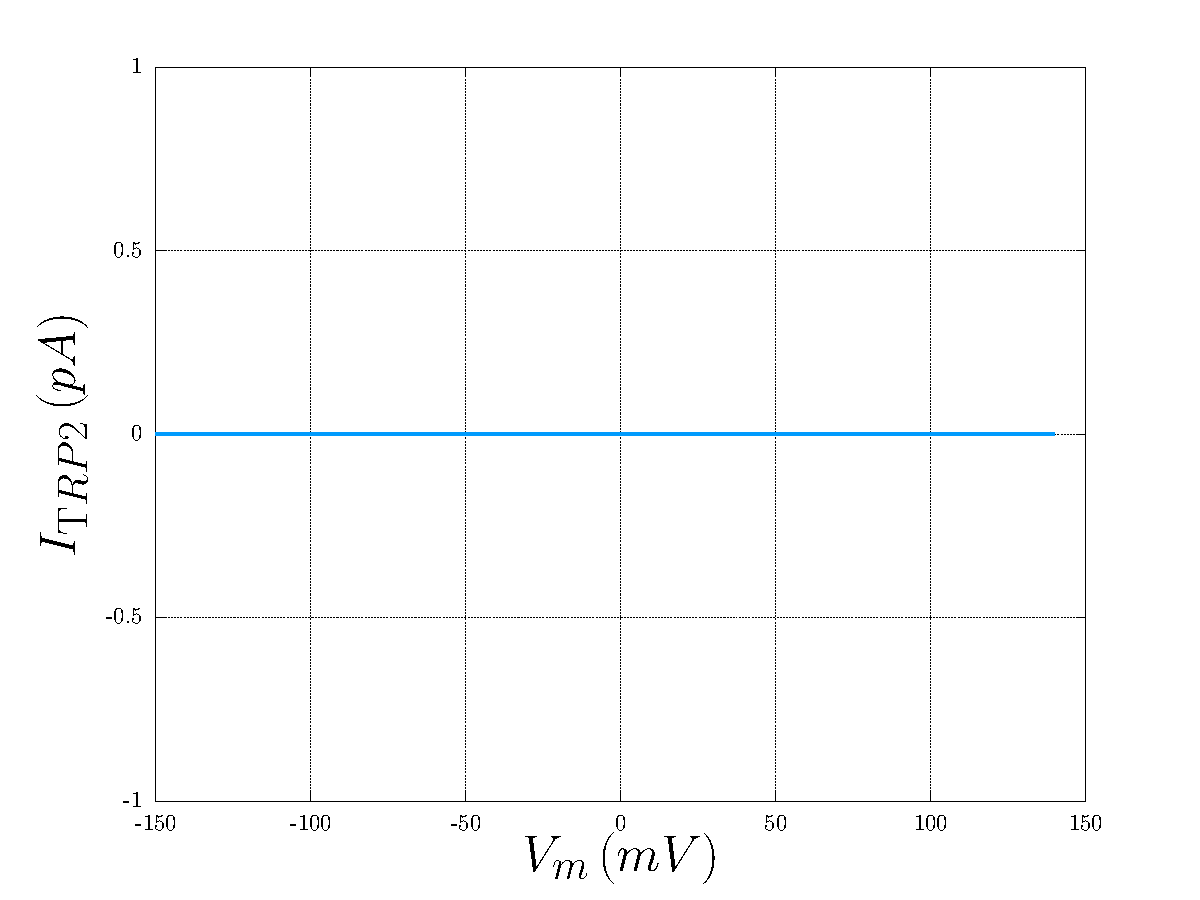
\includegraphics[width=0.36\textwidth]
    {../results/pdf/20110902/V-I_TRP2}}
  \caption{}
  \label{fig:other-currents-vi}
\end{figure}

\clearpage
\begin{figure}
  \centering
  \subfloat{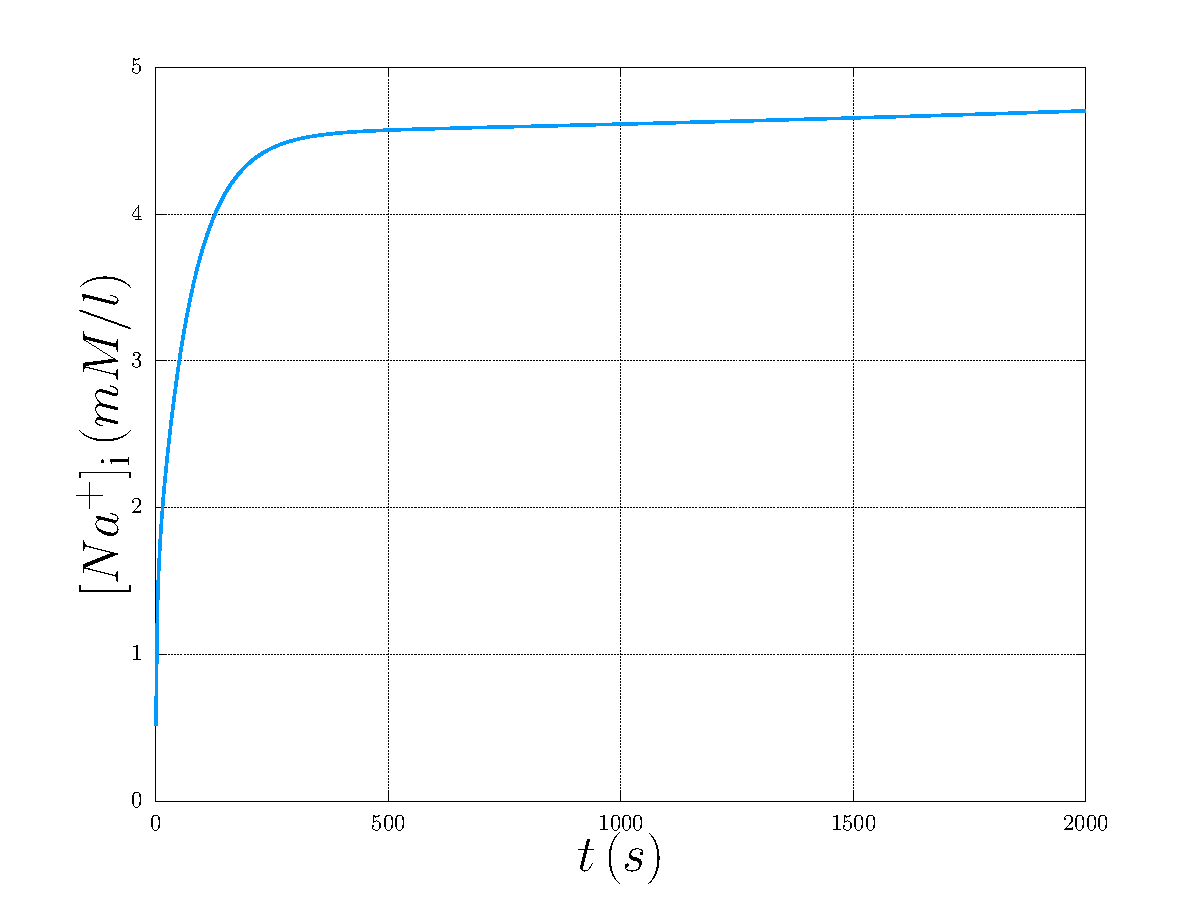
\includegraphics[width=0.3\textwidth]
    {../results/pdf/20110902/t-Na_i}}
  \subfloat{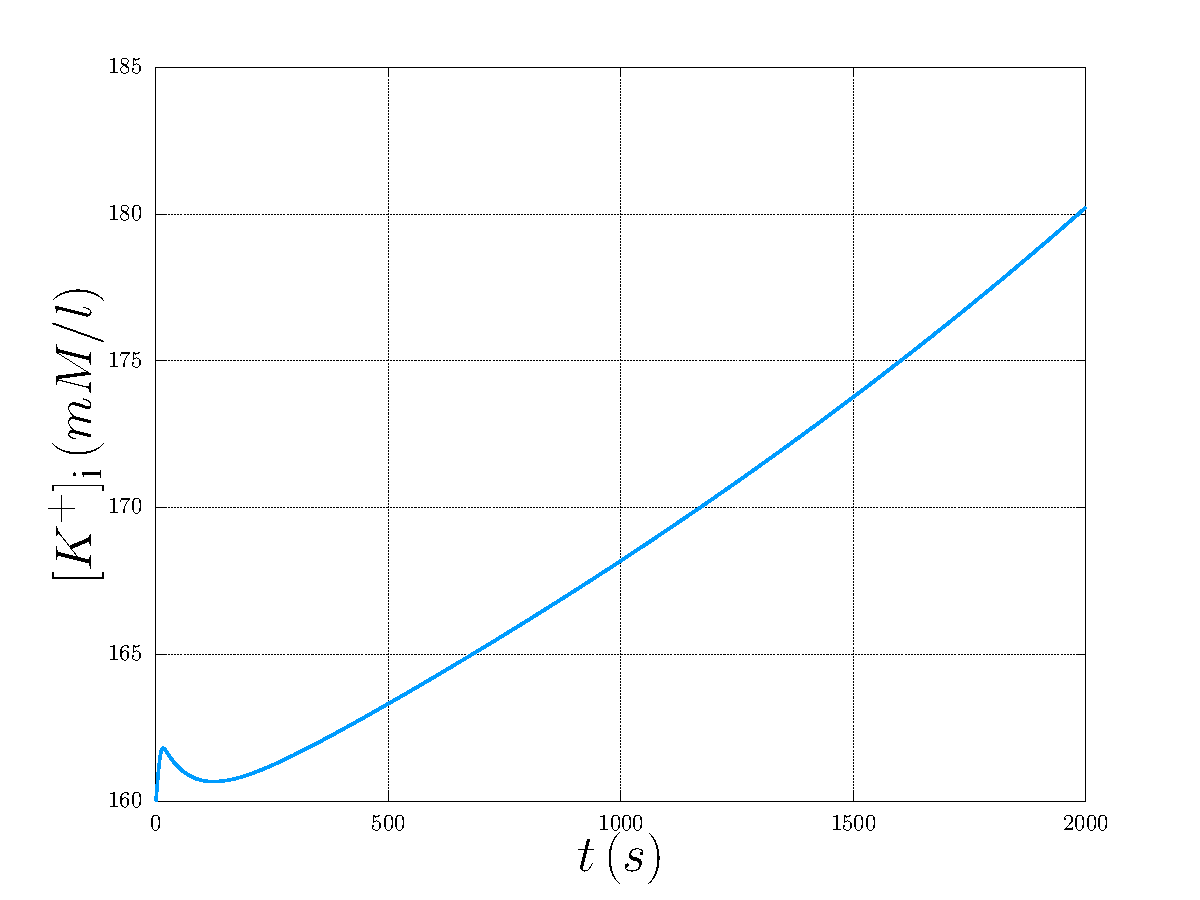
\includegraphics[width=0.3\textwidth]
    {../results/pdf/20110902/t-K_i}}
  \subfloat{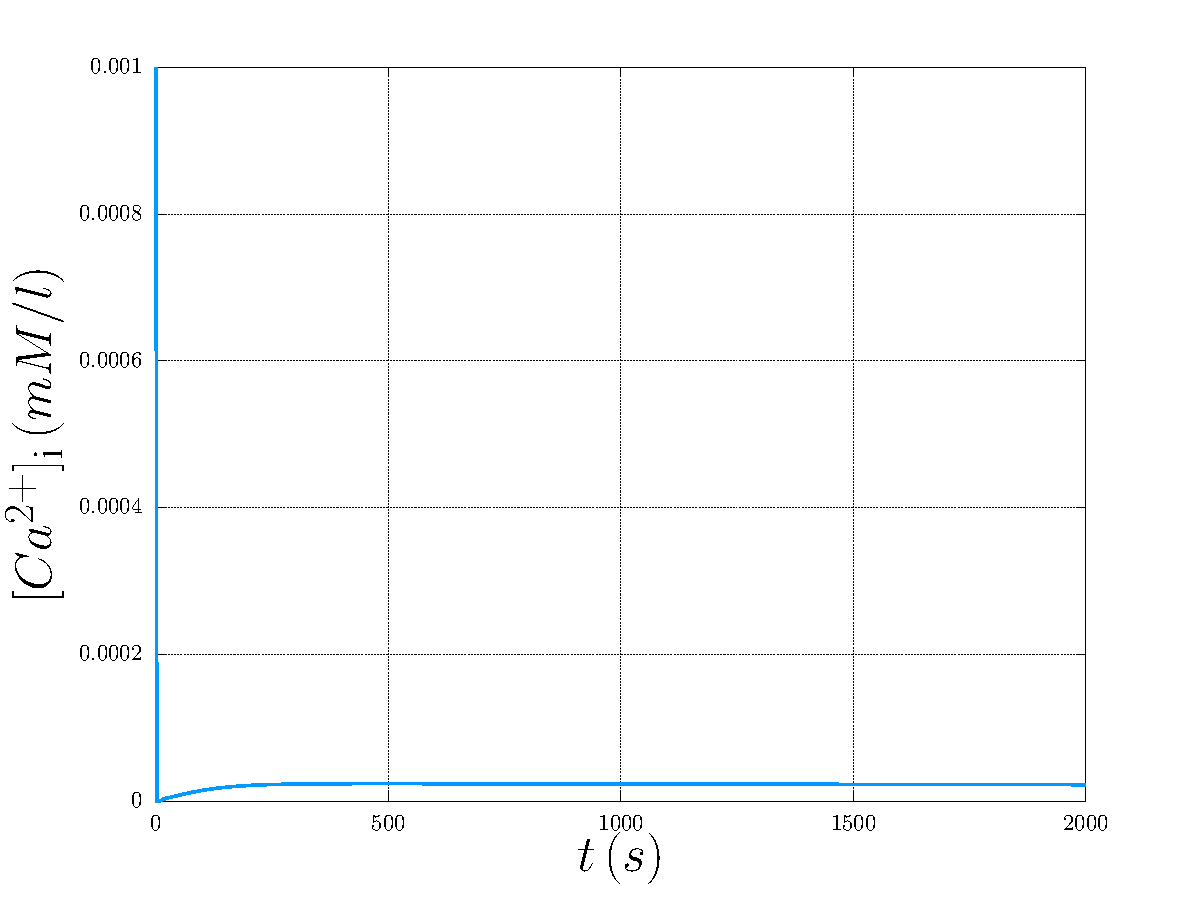
\includegraphics[width=0.3\textwidth]
    {../results/pdf/20110902/t-Ca_i}}\\
  \subfloat{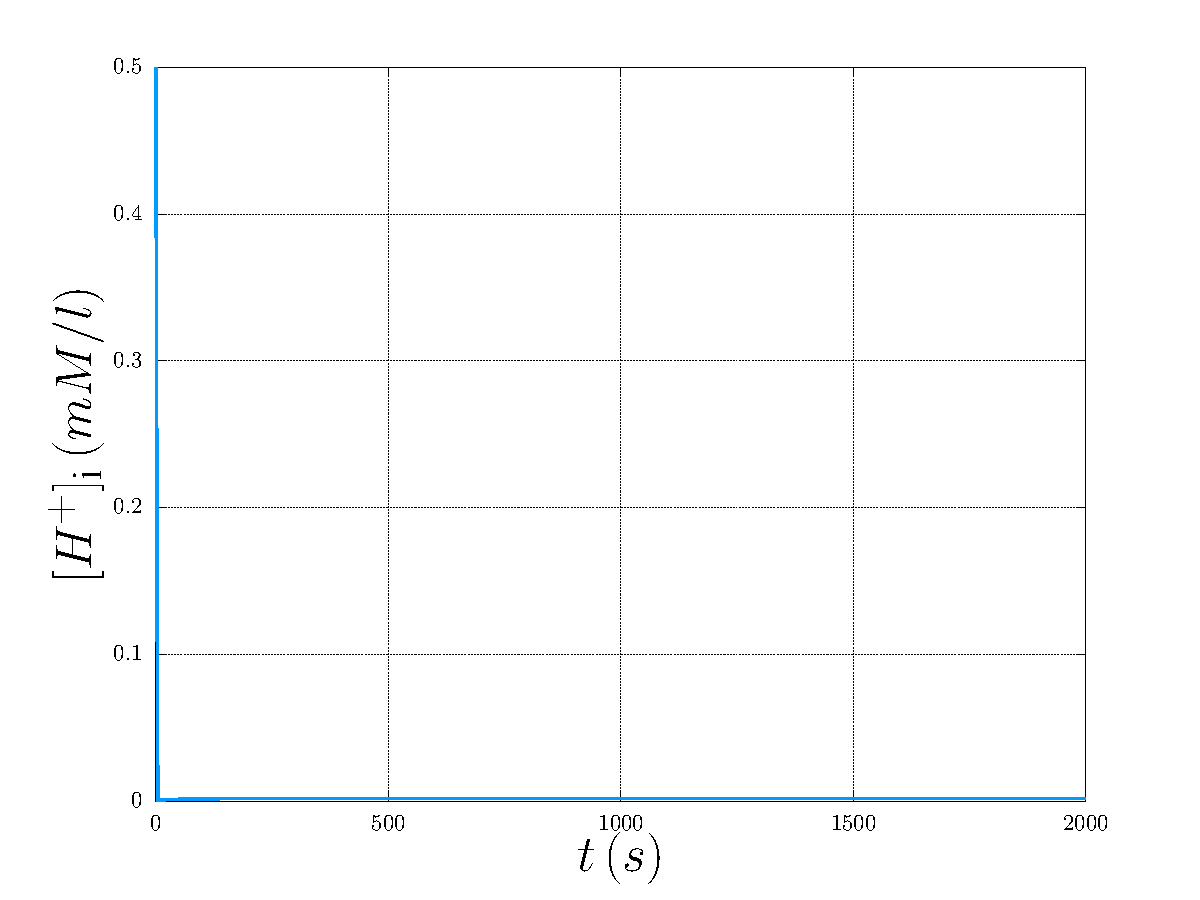
\includegraphics[width=0.3\textwidth]
    {../results/pdf/20110902/t-H_i}}
\subfloat{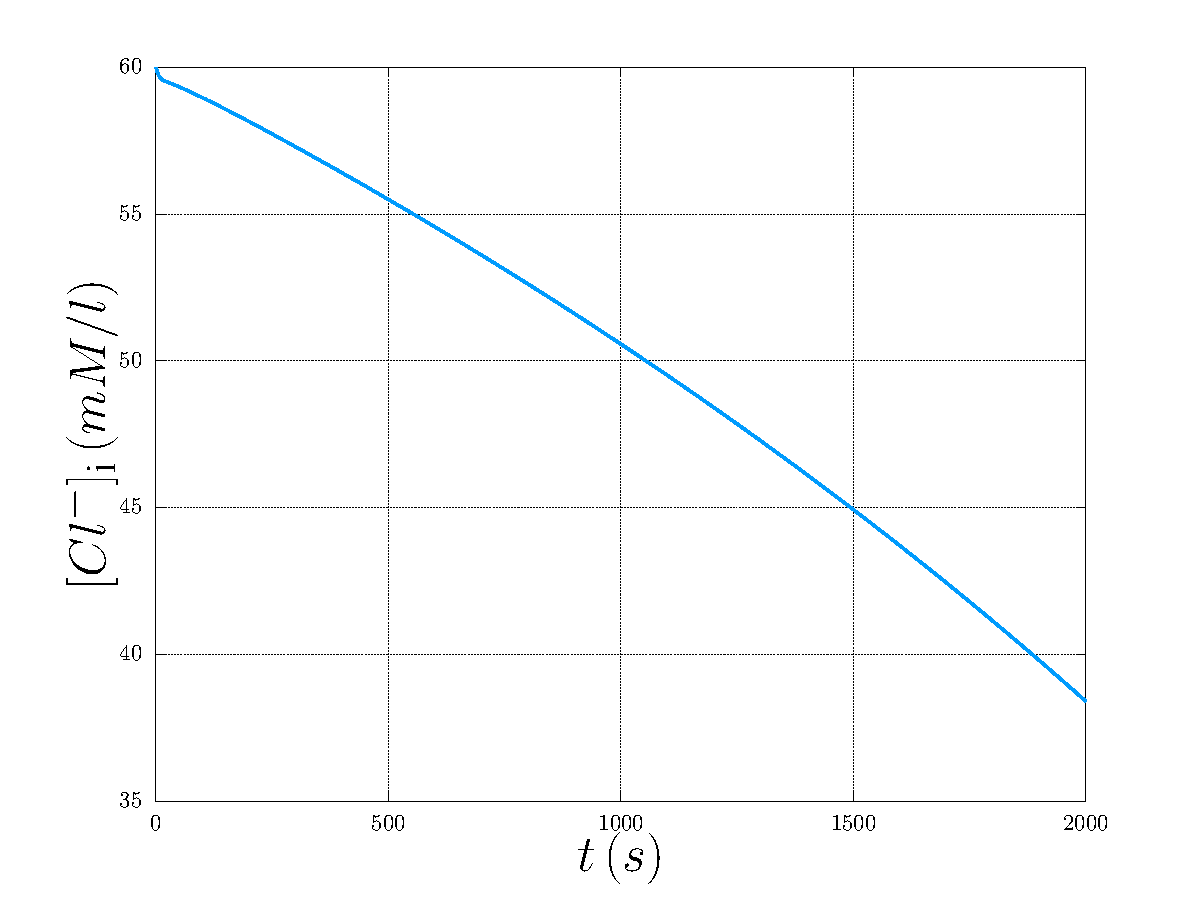
\includegraphics[width=0.3\textwidth]
  {../results/pdf/20110902/t-Cl_i}}
  \subfloat{\hspace{0.3\textwidth}}
  \caption{}
  \label{fig:concentrations}
\end{figure}

\clearpage
\begin{figure}
  \centering
  \subfloat{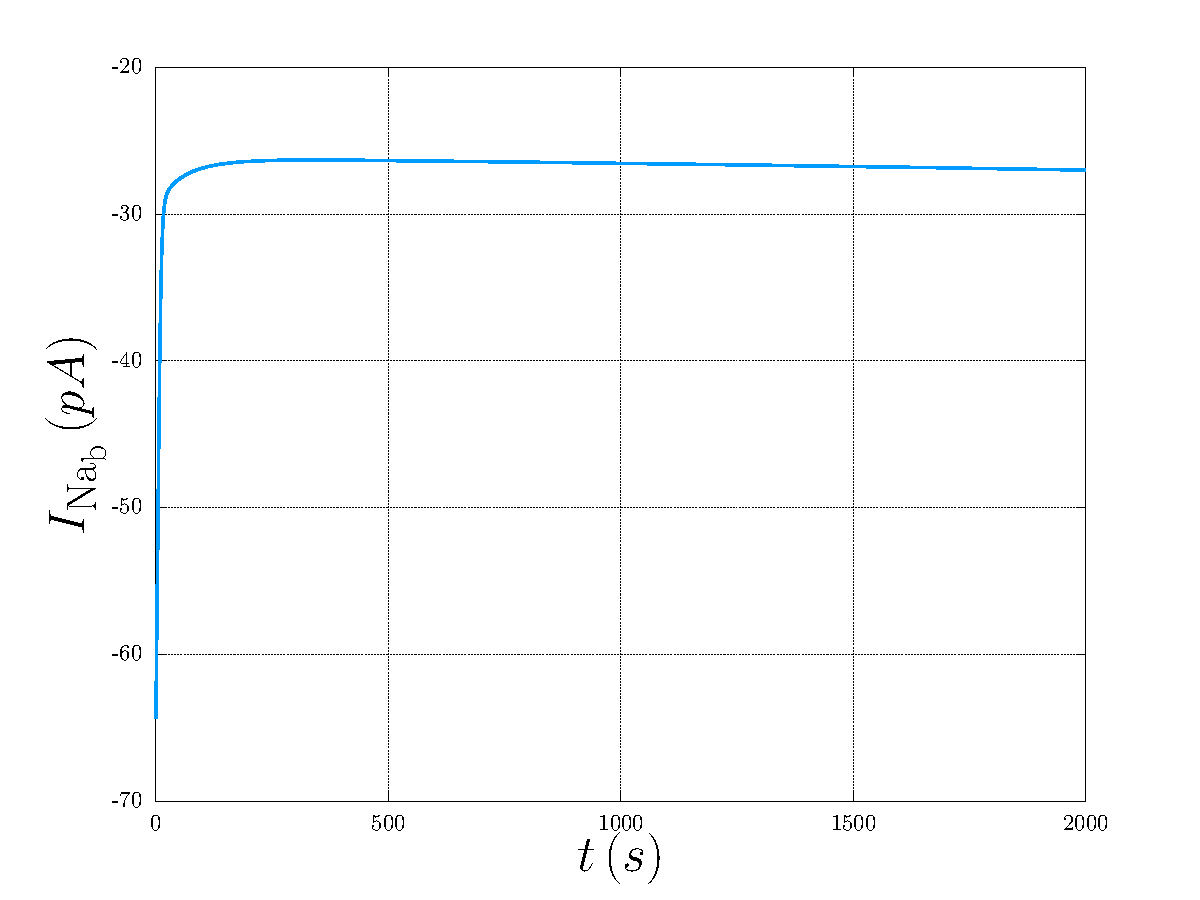
\includegraphics[width=0.36\textwidth]
    {../results/pdf/20110902/t-I_Na_b}}
  \subfloat{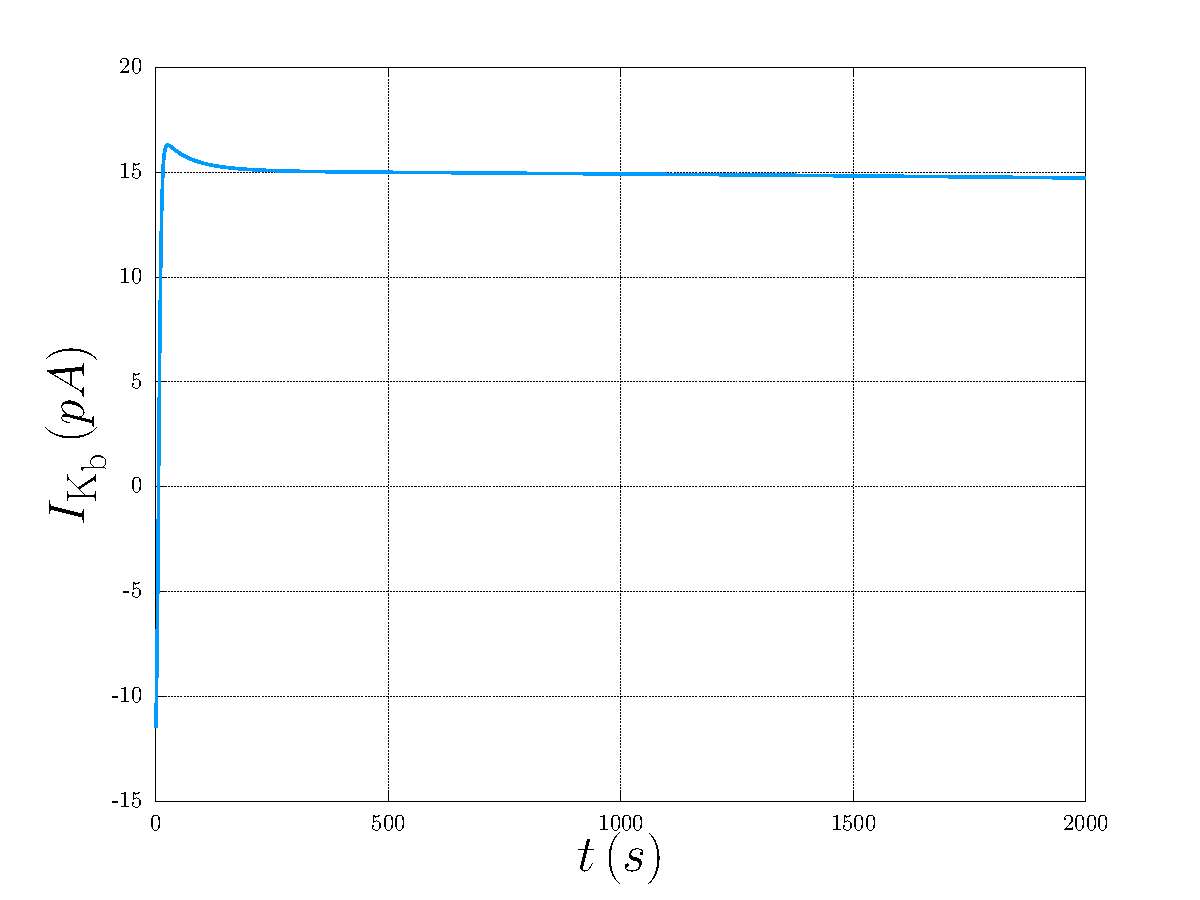
\includegraphics[width=0.36\textwidth]
    {../results/pdf/20110902/t-I_K_b}}\\
  \subfloat{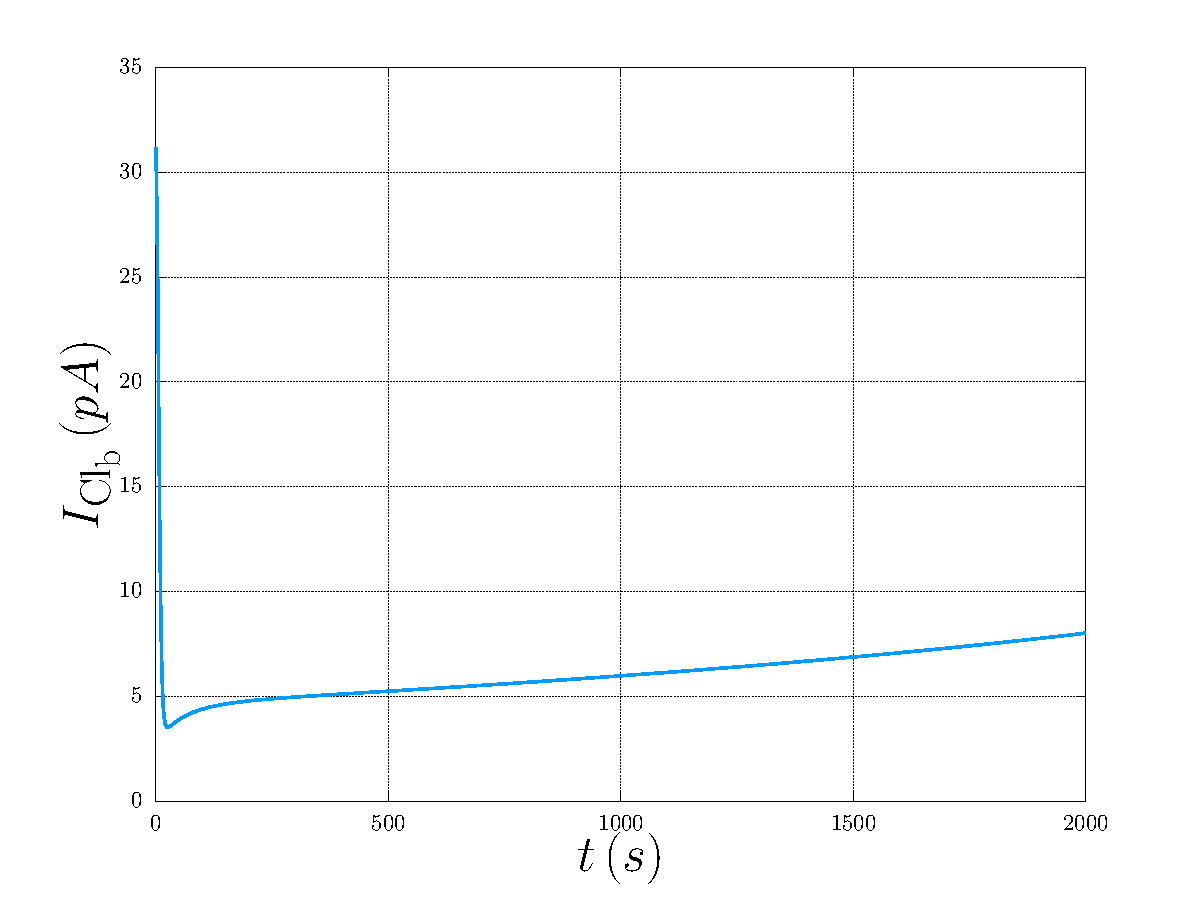
\includegraphics[width=0.36\textwidth]
    {../results/pdf/20110902/t-I_Cl_b}}
  \subfloat{\hspace{0.36\textwidth}}
  \caption{}
  \label{fig:background-currents-ti}
\end{figure}

\clearpage
\begin{figure}
  \centering
  \subfloat{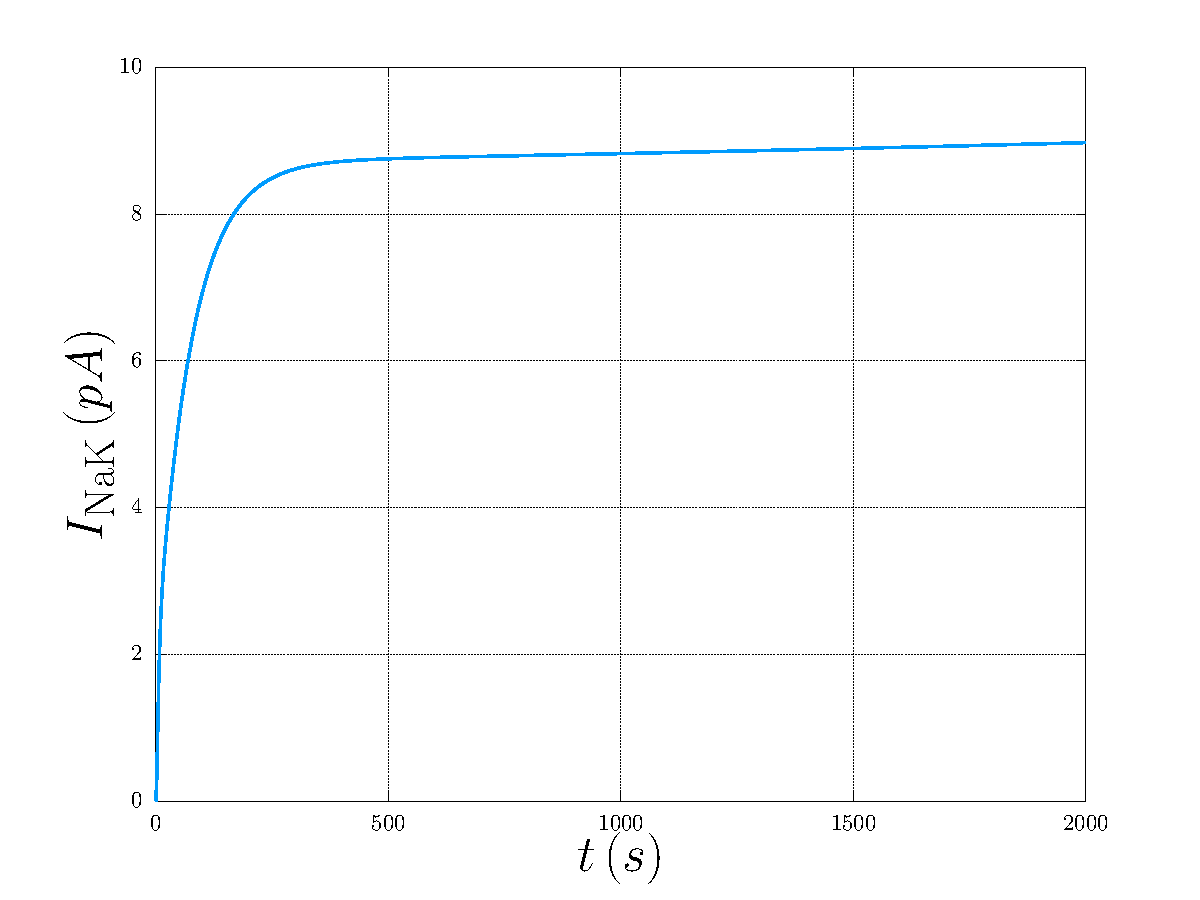
\includegraphics[width=0.36\textwidth]
    {../results/pdf/20110902/t-I_NaK}}
  \subfloat{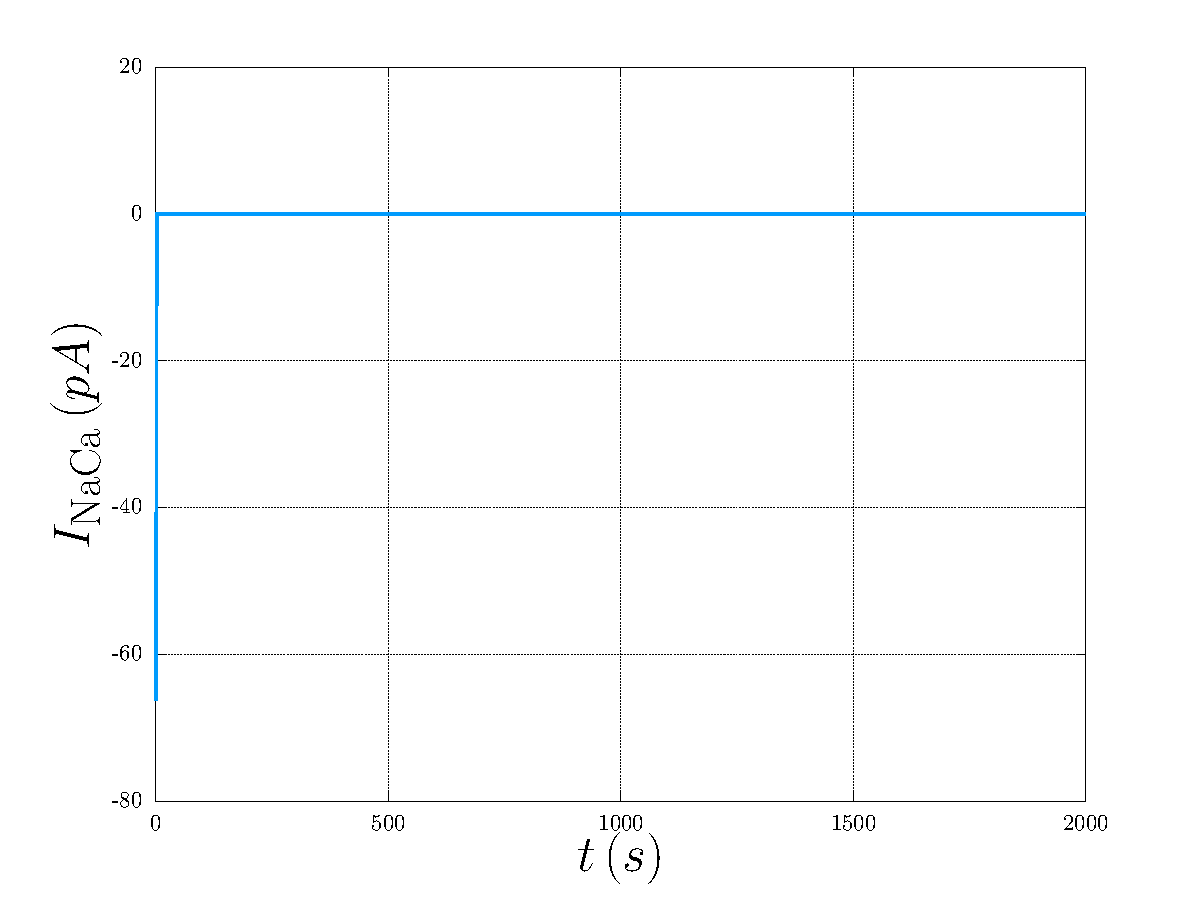
\includegraphics[width=0.36\textwidth]
    {../results/pdf/20110902/t-I_NaCa}}\\
  \subfloat{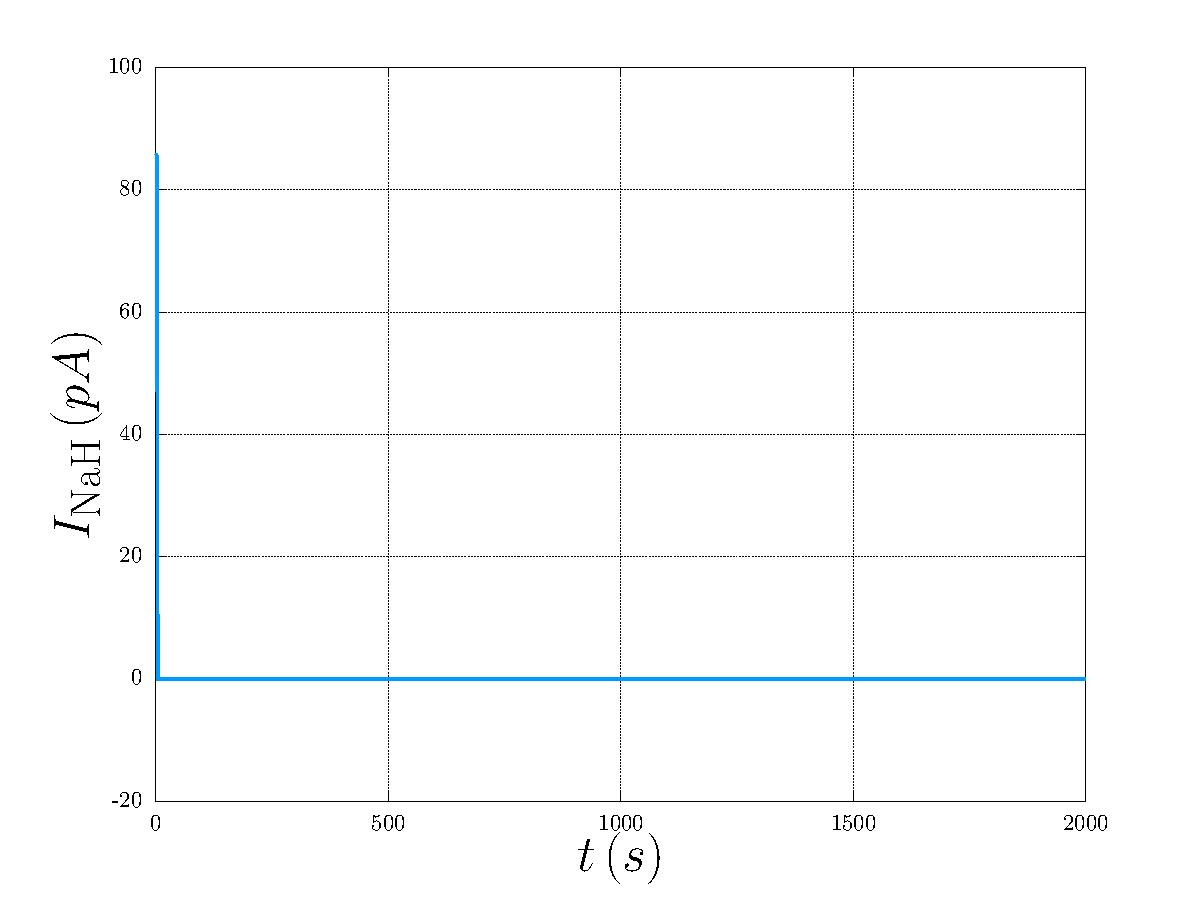
\includegraphics[width=0.36\textwidth]
    {../results/pdf/20110902/t-I_NaH}}
  \subfloat{\hspace{0.36\textwidth}}
  \caption{}
  \label{fig:pumps-and-exchangers-ti}
\end{figure}

\clearpage
\begin{figure}
  \centering
  \subfloat{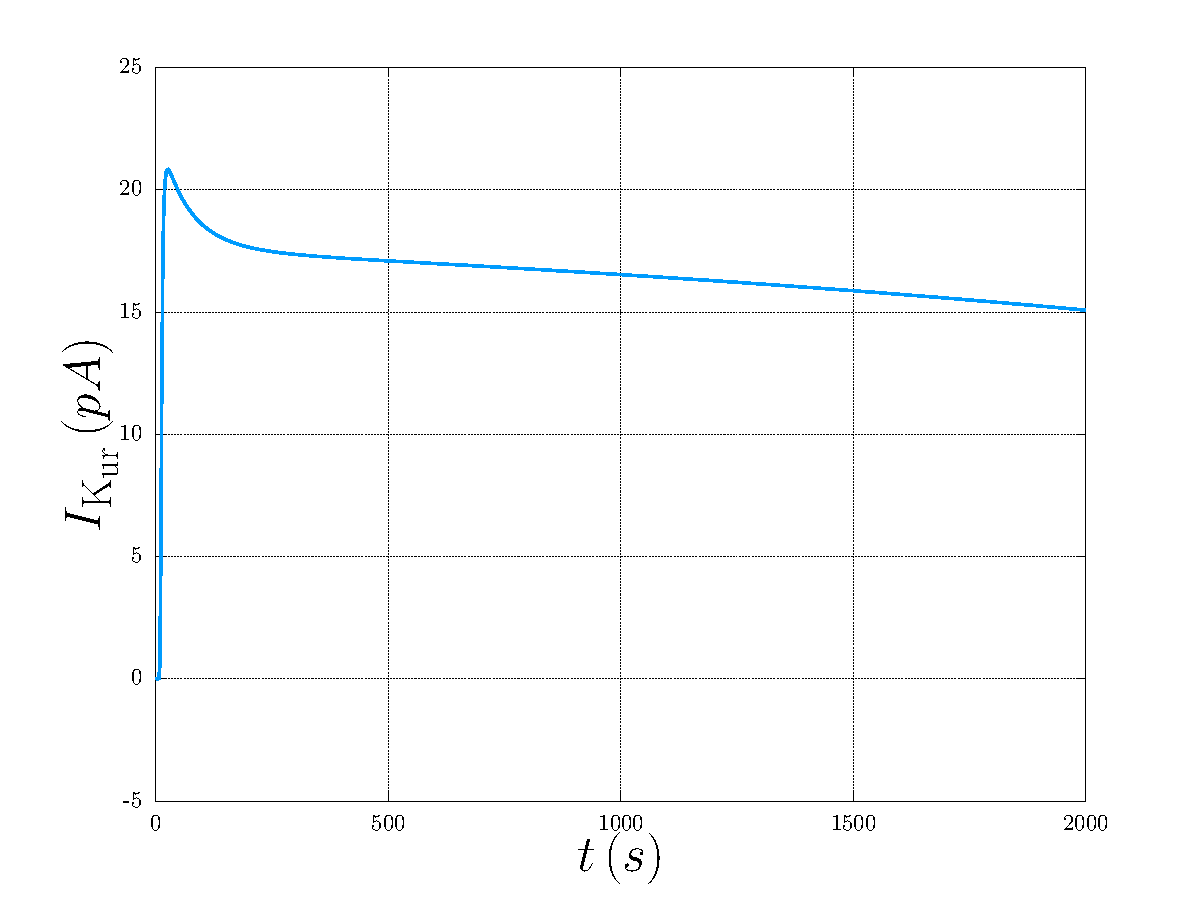
\includegraphics[width=0.36\textwidth]
    {../results/pdf/20110902/t-I_K_ur}}
  \subfloat{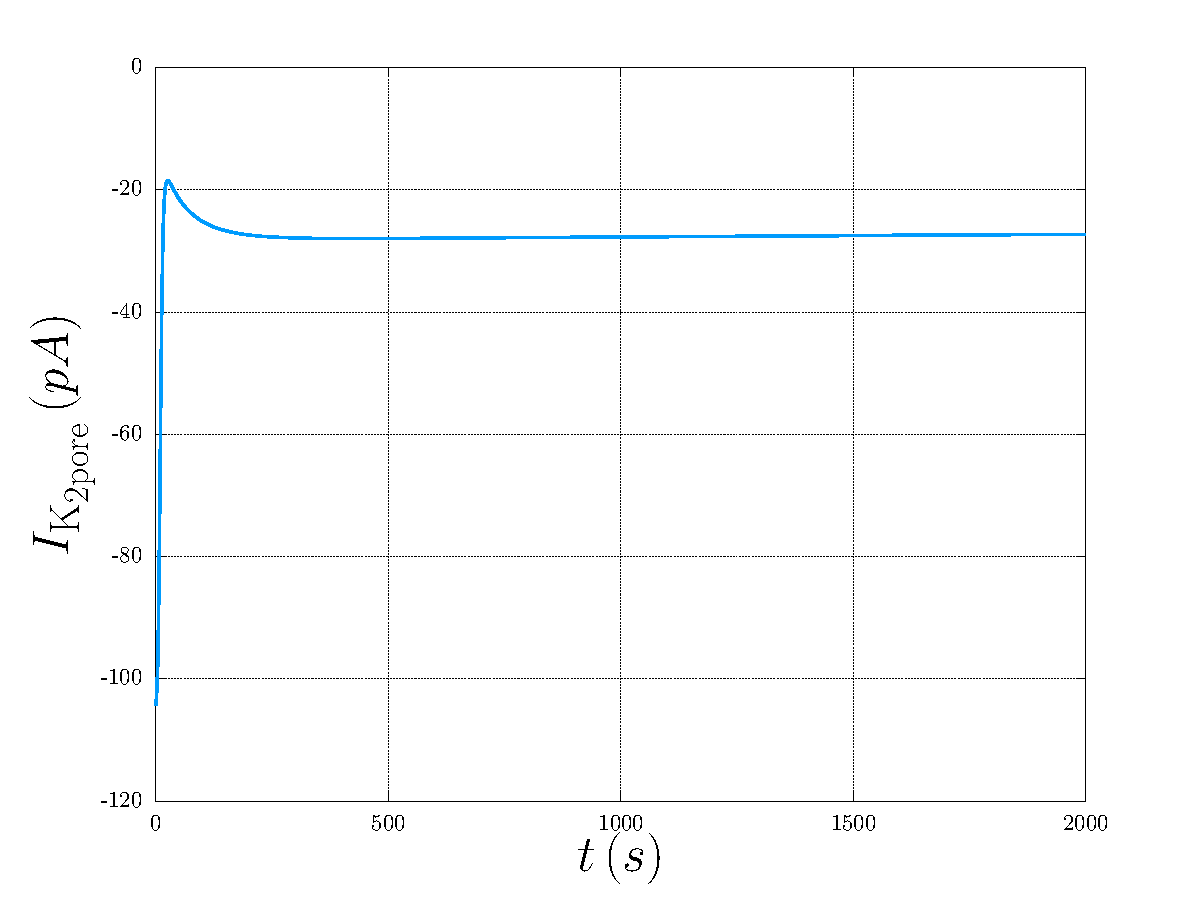
\includegraphics[width=0.36\textwidth]
    {../results/pdf/20110902/t-I_K_2pore}}\\
  \subfloat{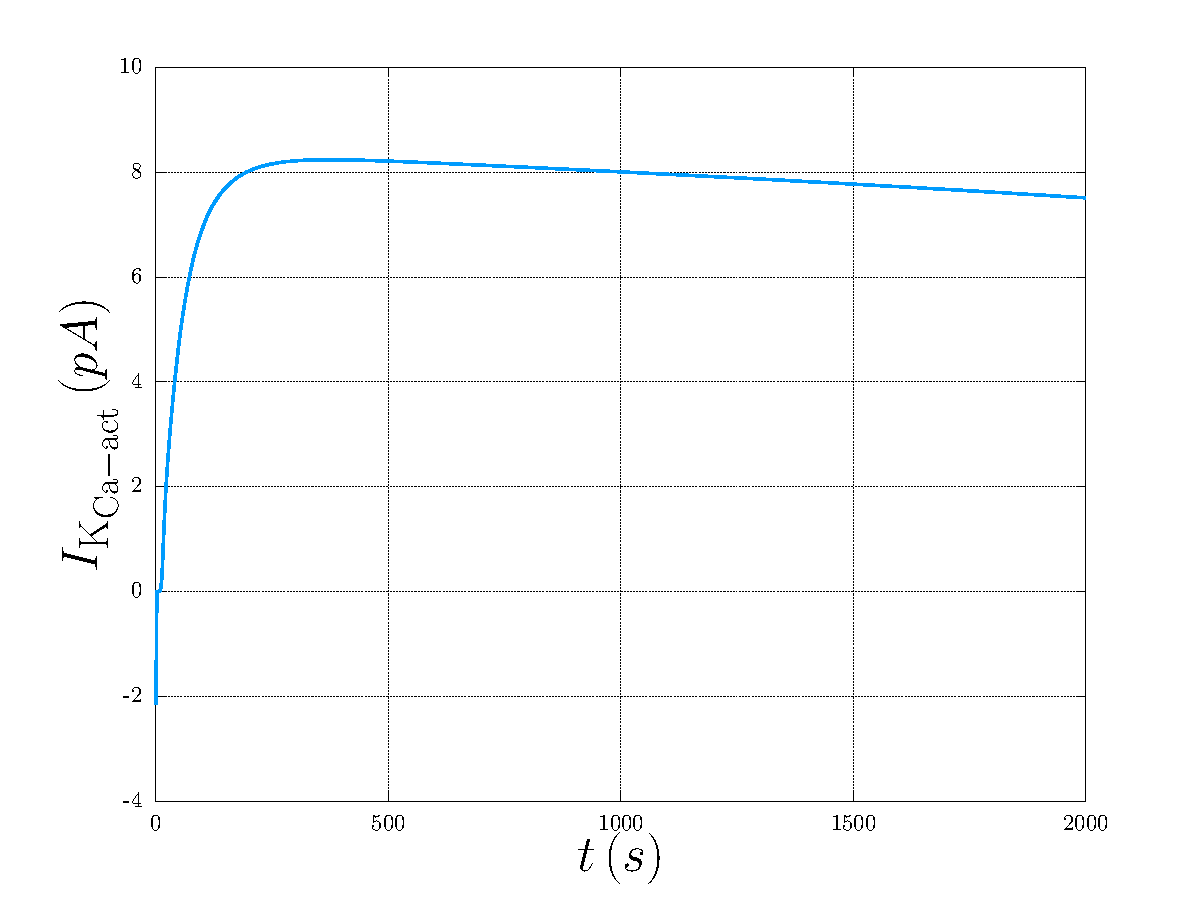
\includegraphics[width=0.36\textwidth]
    {../results/pdf/20110902/t-I_K_Ca_act}}
  \subfloat{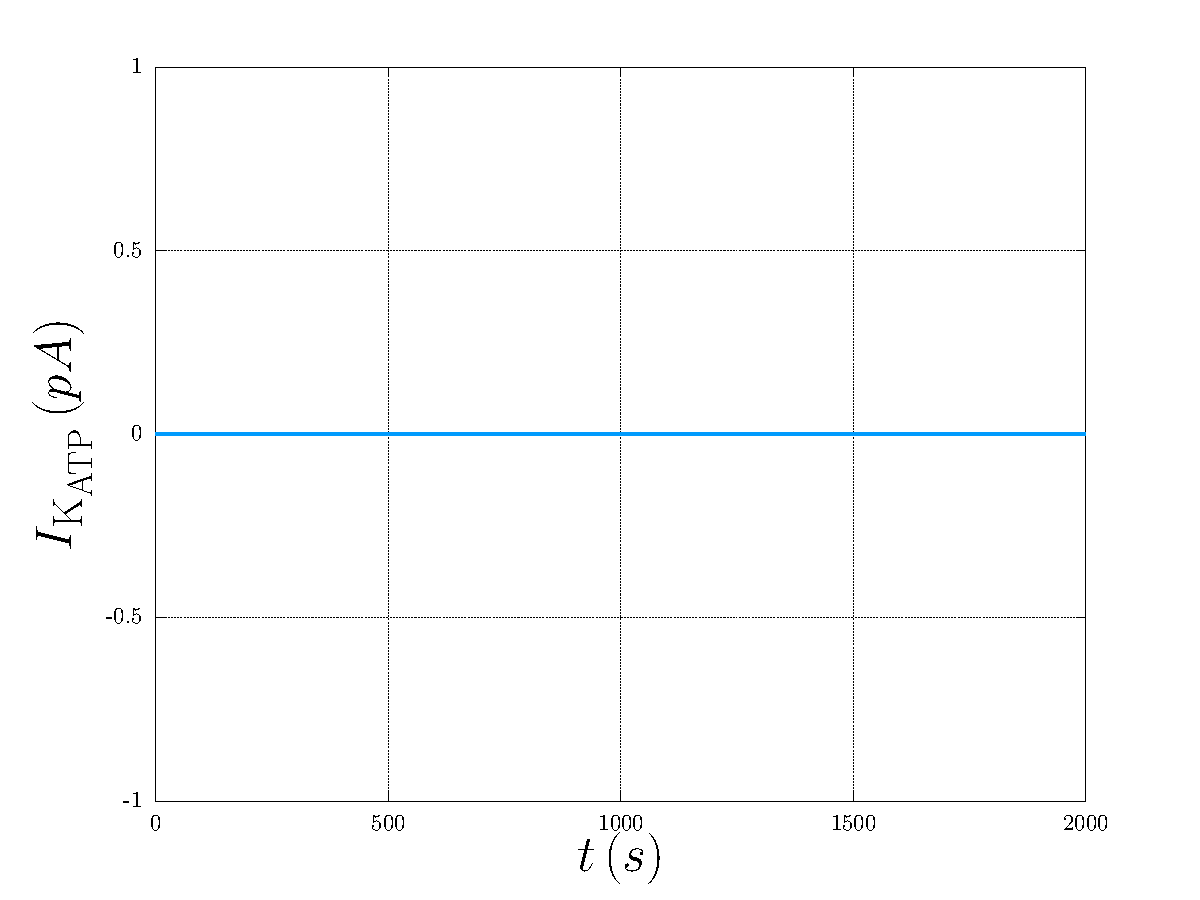
\includegraphics[width=0.36\textwidth]
    {../results/pdf/20110902/t-I_K_ATP}}
  \caption{}
  \label{fig:potassium-currents-ti}
\end{figure}

\clearpage
\begin{figure}
  \centering
  \subfloat{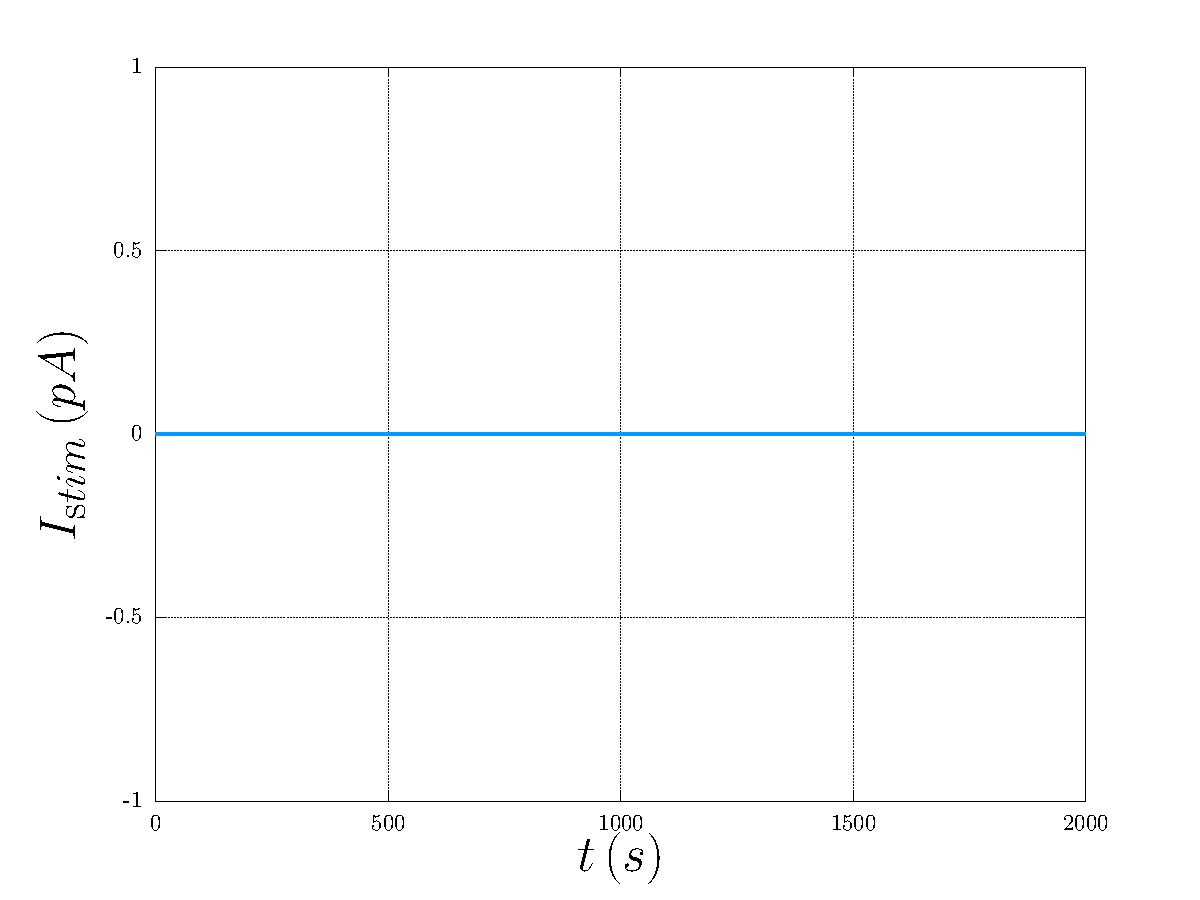
\includegraphics[width=0.36\textwidth]
    {../results/pdf/20110902/t-I_stim}}
  \subfloat{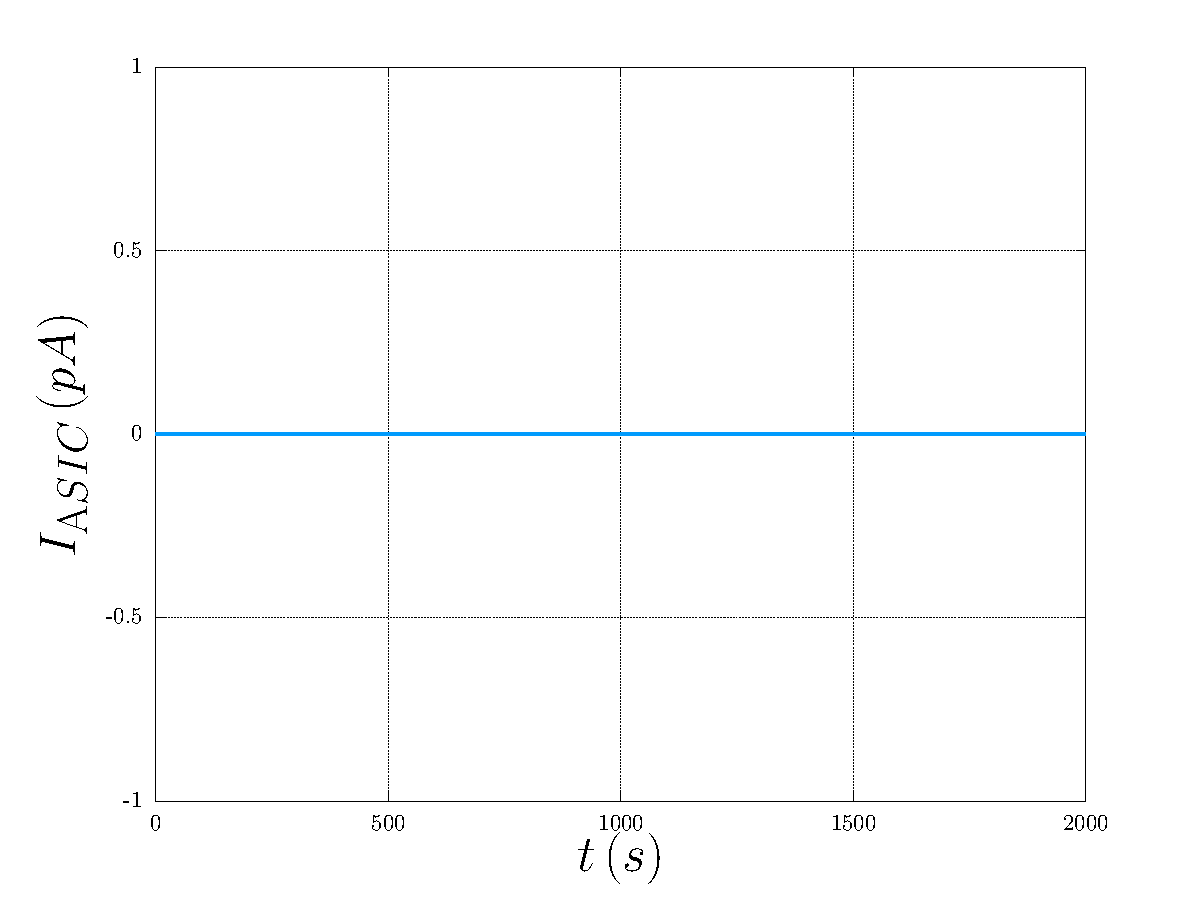
\includegraphics[width=0.36\textwidth]
    {../results/pdf/20110902/t-I_ASIC}}\\
  \subfloat{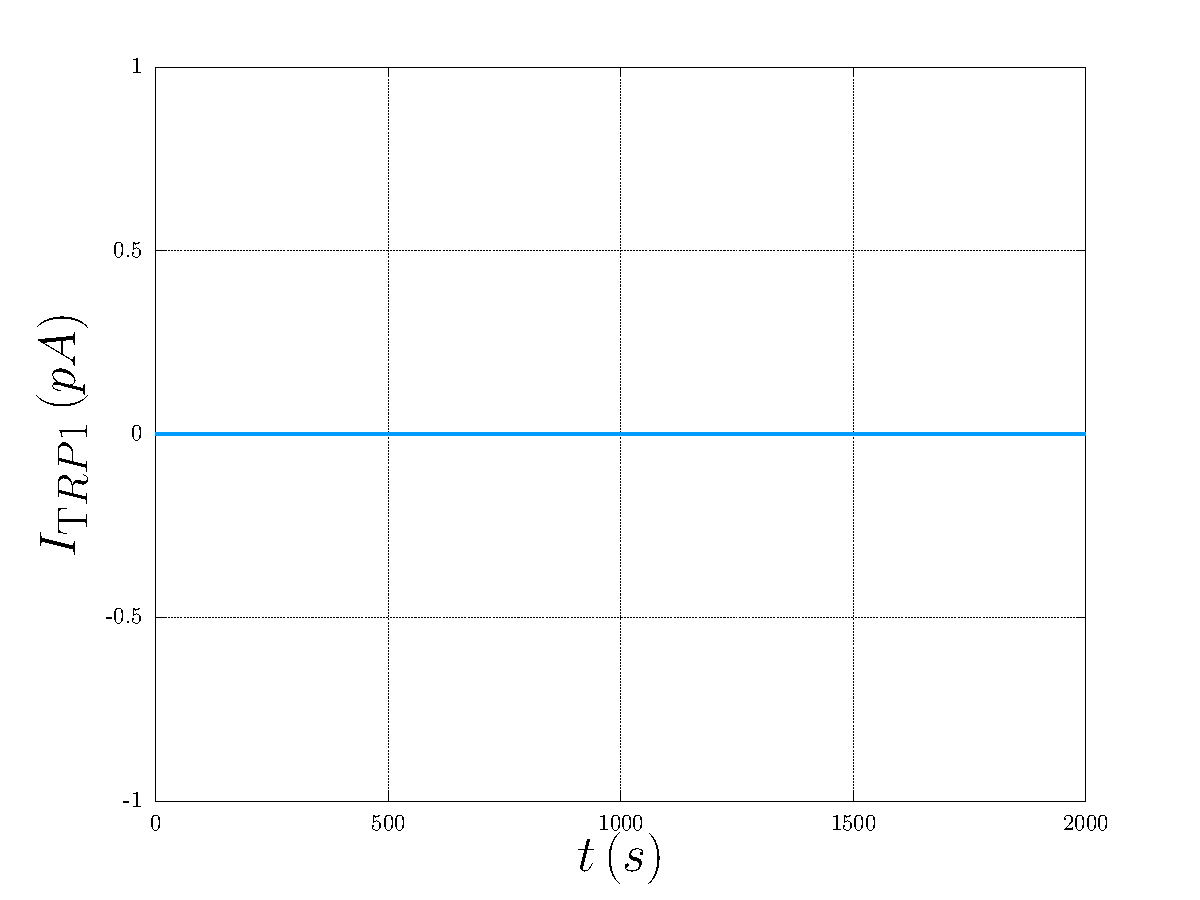
\includegraphics[width=0.36\textwidth]
    {../results/pdf/20110902/t-I_TRP1}}
  \subfloat{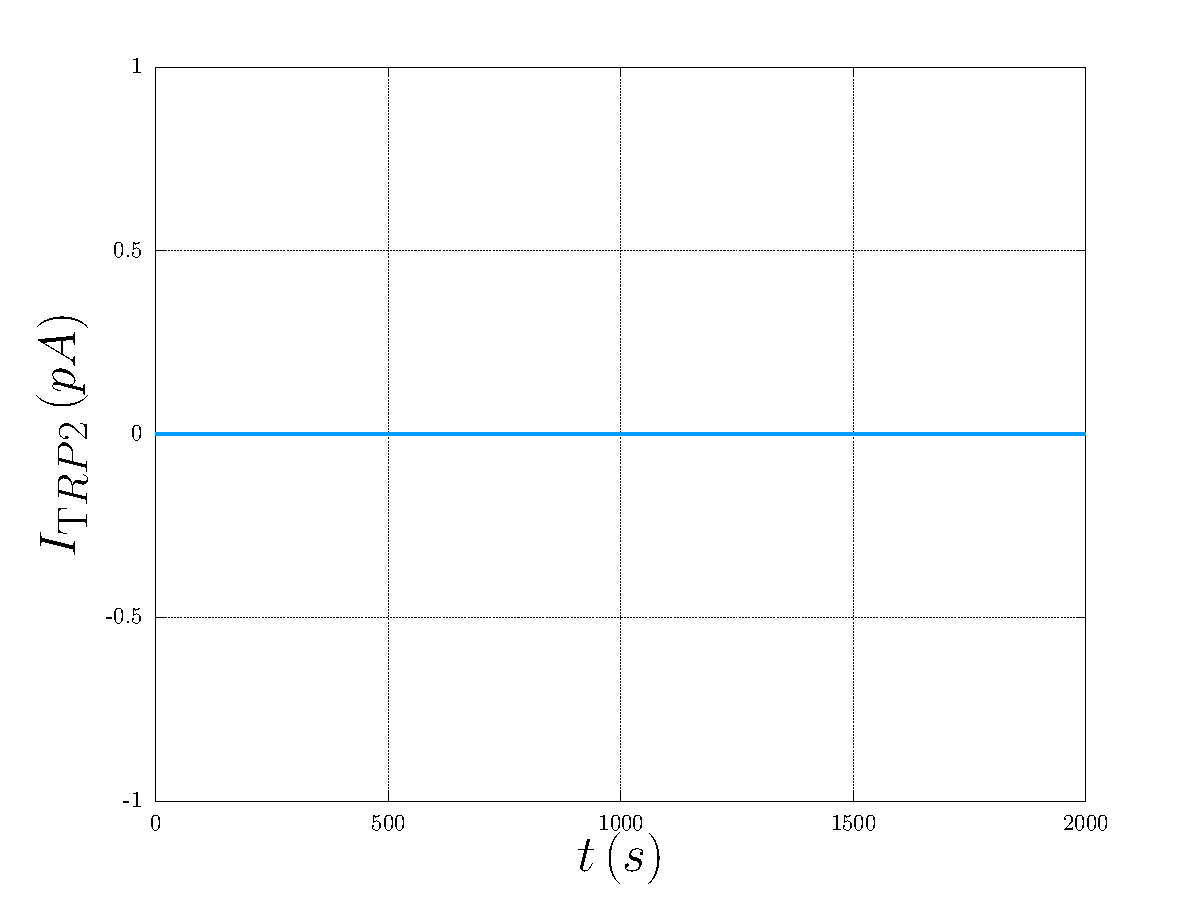
\includegraphics[width=0.36\textwidth]
    {../results/pdf/20110902/t-I_TRP2}}
  \caption{}
  \label{fig:other-currents-ti}
\end{figure}

\clearpage
\begin{figure}
  \centering
  \subfloat{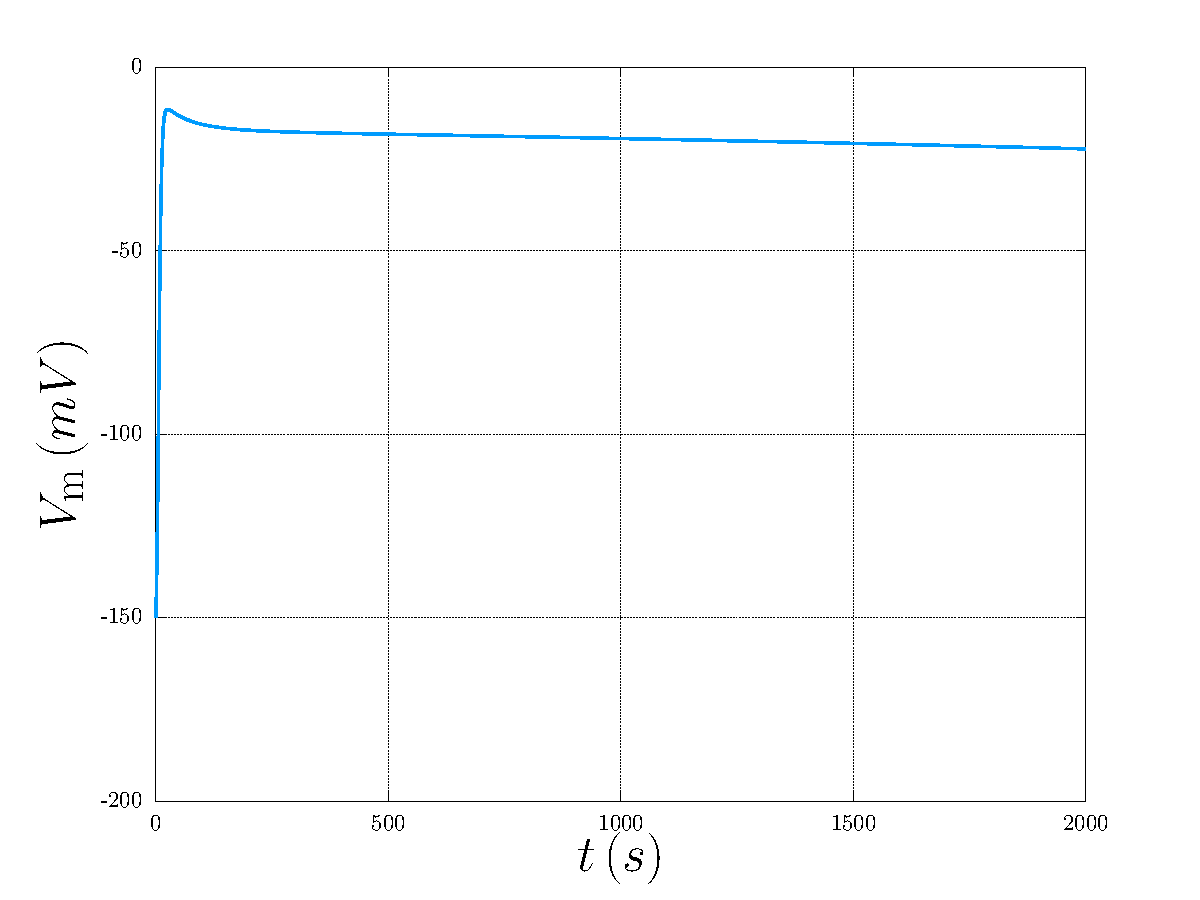
\includegraphics[width=0.36\textwidth]
    {../results/pdf/20110902/t-V}}
  \subfloat{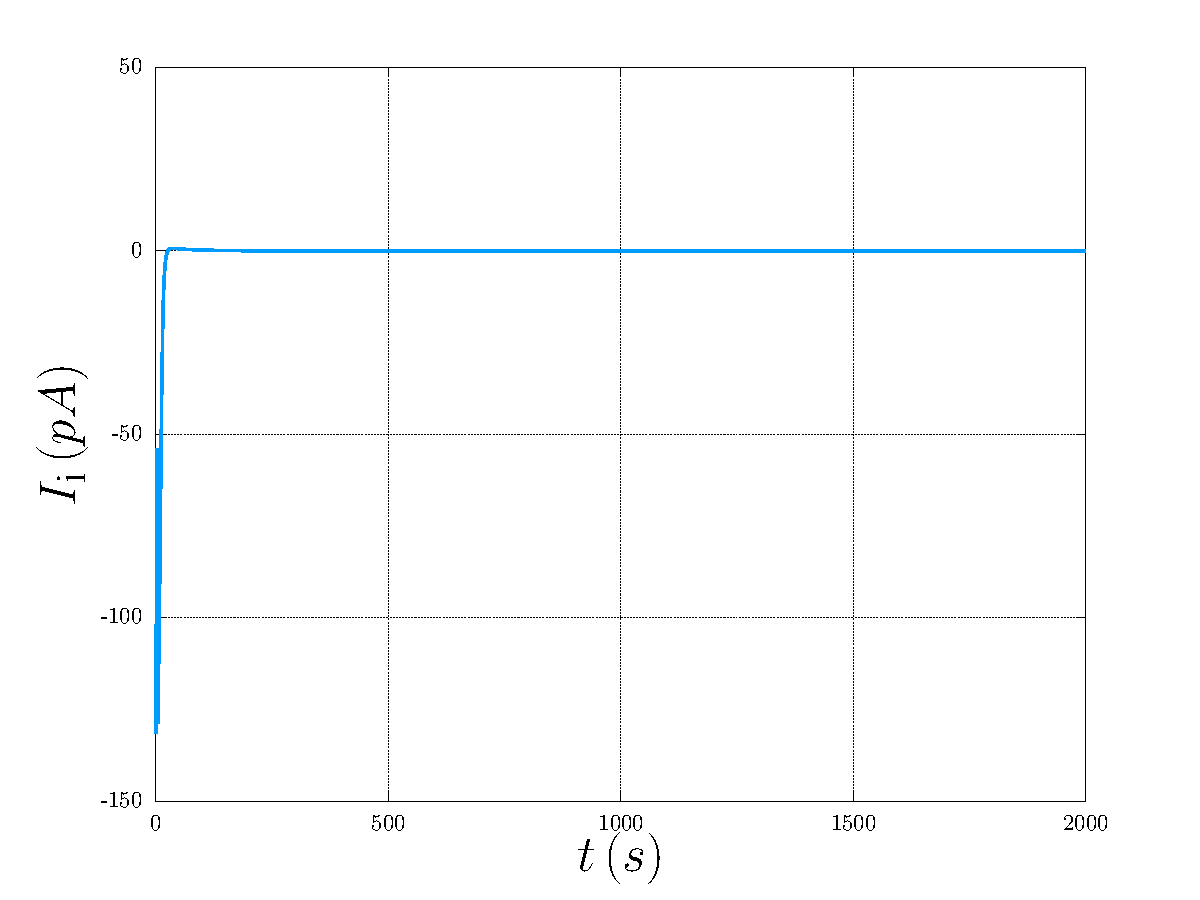
\includegraphics[width=0.36\textwidth]
    {../results/pdf/20110902/t-I_i}}\\
  \subfloat{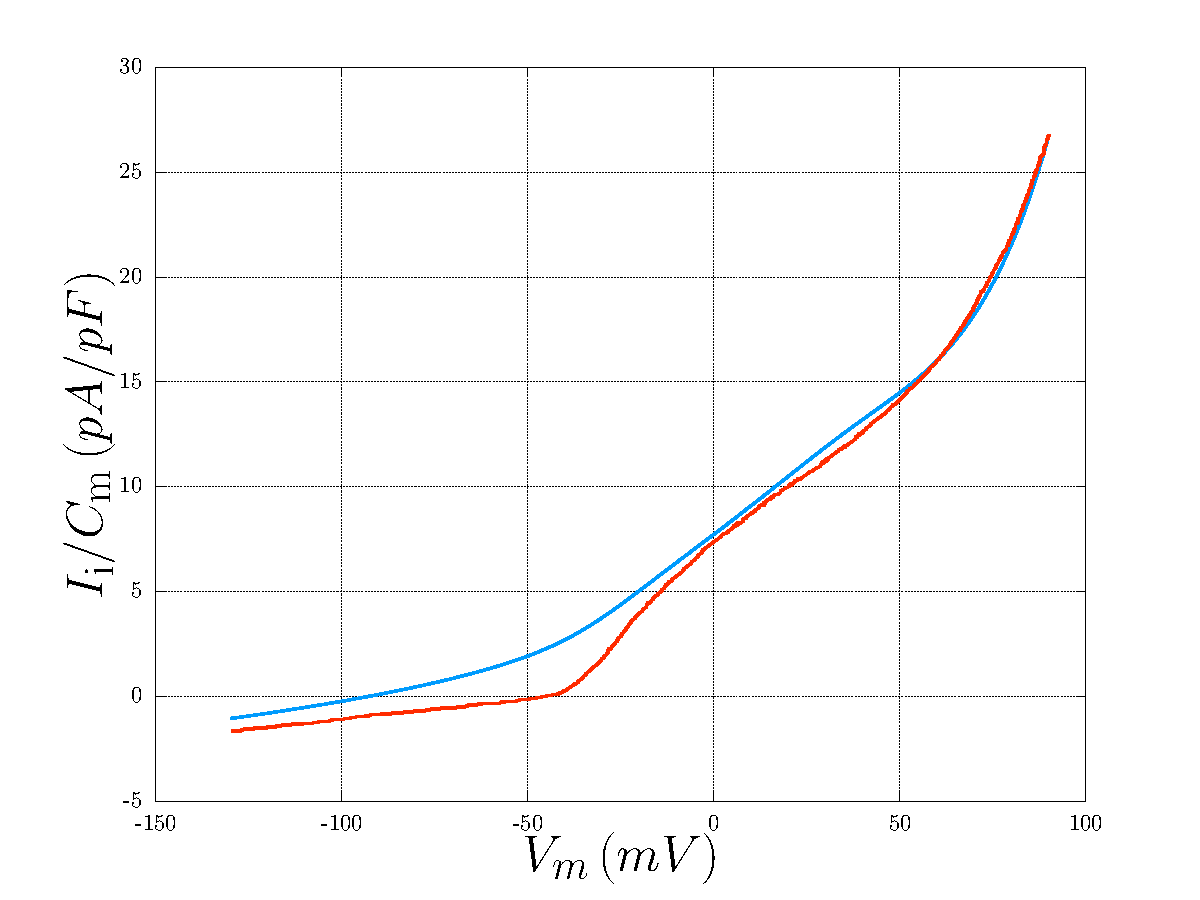
\includegraphics[width=0.36\textwidth]
    {../results/pdf/20110902/V-I_i_by_Cm}}
  \subfloat{\hspace{0.36\textwidth}}
  \caption{}
  \label{fig:overall-behaviour}
\end{figure}

\clearpage
\begin{figure}
  \centering
  \subfloat[Without BUP]{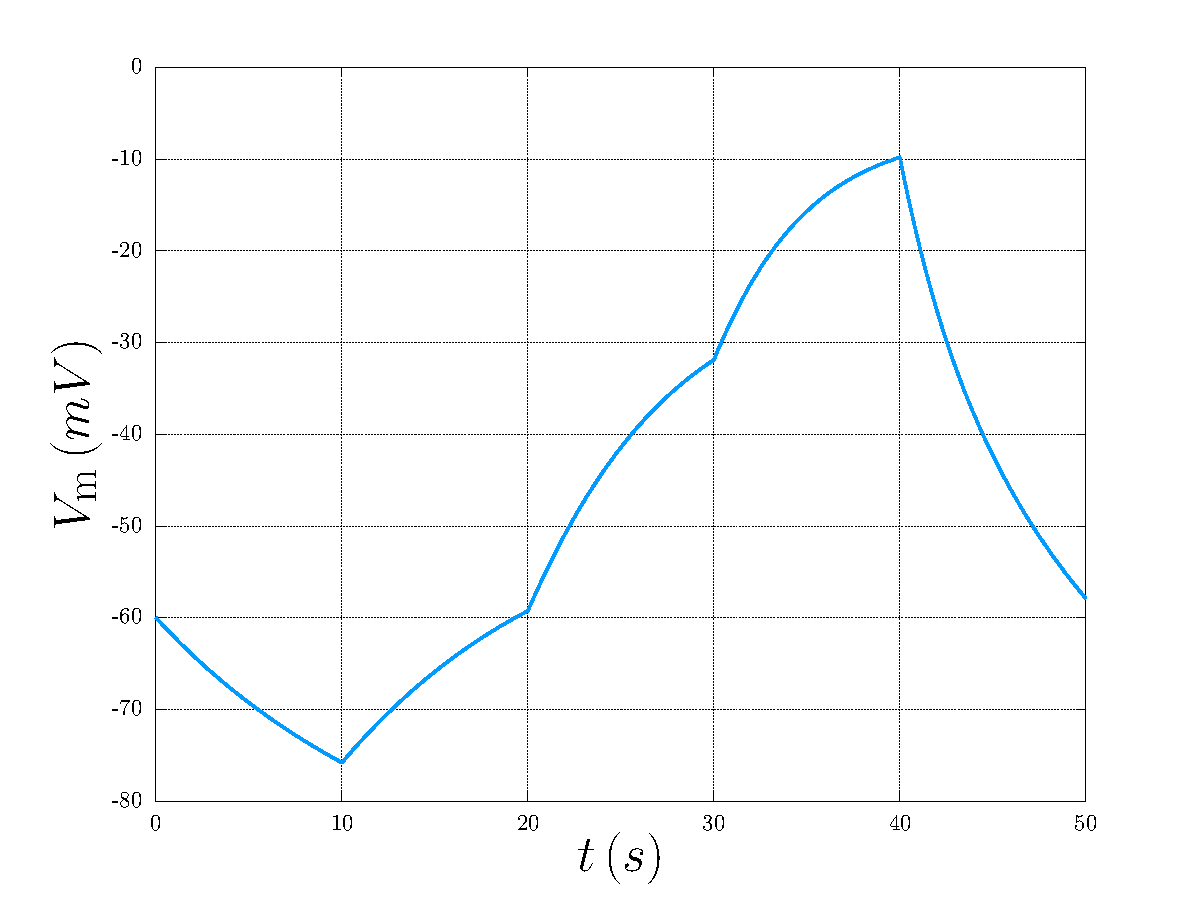
\includegraphics[width=0.36\textwidth]
    {../results/pdf/20110902/t-V-withoutBUP}}
  \subfloat[With BUP]{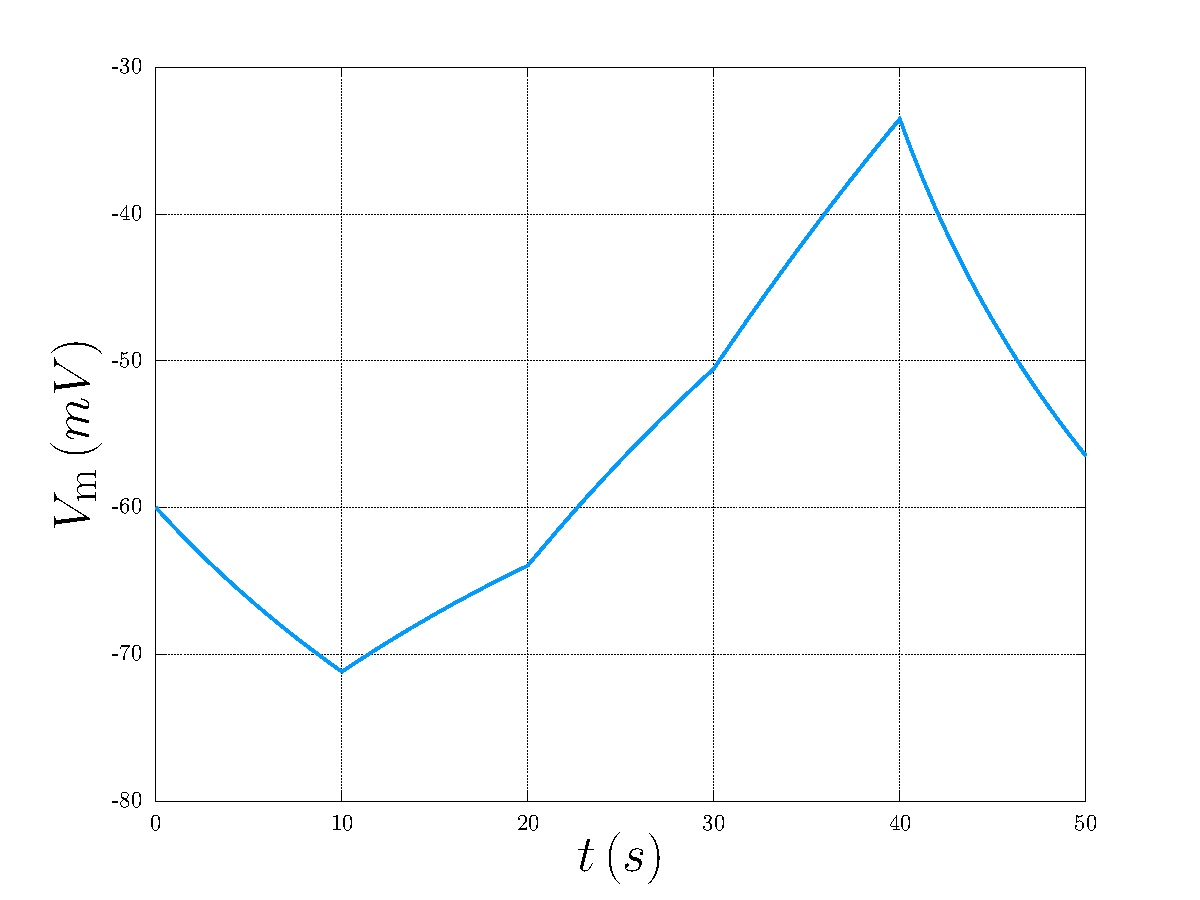
\includegraphics[width=0.36\textwidth]
    {../results/pdf/20110902/t-V-withBUP}}\\
  \subfloat{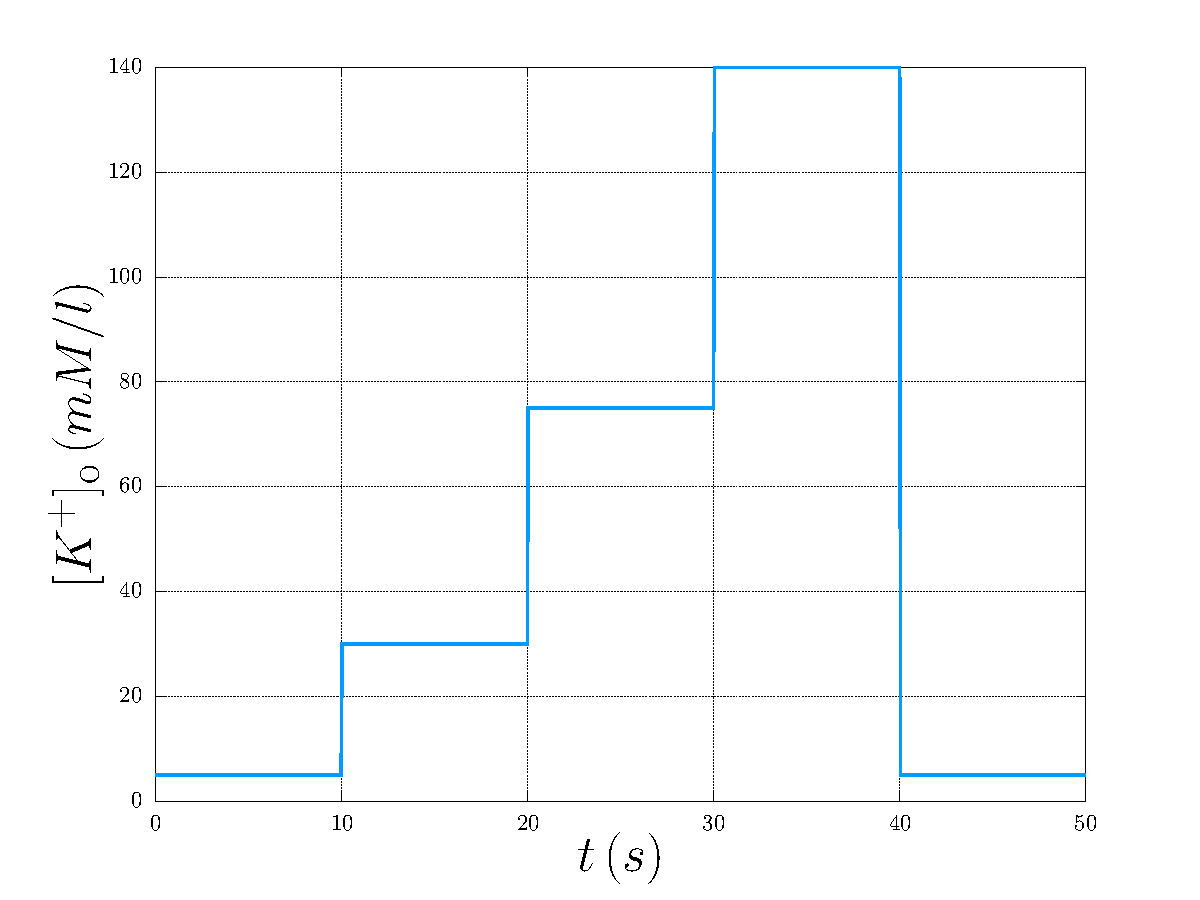
\includegraphics[width=0.36\textwidth]
    {../results/pdf/20110902/t-K_o}}
  \subfloat{\hspace{0.36\textwidth}}
  \caption{}
  \label{fig:varying-Ko}
\end{figure}

% Local Variables:
% TeX-master: "chondrocyte-model"
% mode: latex
% mode: flyspell
% End: